%http://www.daniel-brettschneider.de/allgemein/latex-vorlage-fur-hausarbeiten-oder-abschlussarbeiten

\documentclass[12pt,a4paper,bibliography=totocnumbered,listof=totocnumbered]{scrartcl}
\usepackage[ngerman]{babel}
\usepackage[utf8]{inputenc}
\usepackage{amsmath}
\usepackage{amsfonts}
\usepackage{amssymb}
\usepackage{graphicx}
\usepackage{fancyhdr}
\usepackage{tabularx}
\usepackage{geometry}
\usepackage{setspace}
\usepackage[right]{eurosym}
\usepackage[printonlyused]{acronym}
\usepackage{subfig}
\usepackage{floatflt}
\usepackage{float}
\usepackage{placeins}
\usepackage[usenames,dvipsnames]{color}
\usepackage{colortbl}
\usepackage{paralist}
\usepackage{array}
\usepackage{titlesec}
\usepackage{parskip}
\usepackage{booktabs}
\usepackage[right]{eurosym}
%\usepackage{picins}
\usepackage[subfigure,titles]{tocloft}
\usepackage[pdfpagelabels=true]{hyperref}
\usepackage{listings}
\usepackage{colortbl}
\lstset{language=C}  


%für Listings
\usepackage{listings}
\lstset{basicstyle=\footnotesize, captionpos=b, breaklines=true, showstringspaces=false, tabsize=2, frame=lines, numbers=left, numberstyle=\tiny, xleftmargin=2em, framexleftmargin=2em}
\makeatletter
\def\l@lstlisting#1#2{\@dottedtocline{1}{0em}{1em}{\hspace{1,5em} Lst. #1}{#2}}
\makeatother




\newcommand{\includecode}[1]{\lstinputlisting[caption=#1]{#1}}

%Seitenränder
\geometry{a4paper, top=27mm, left=30mm, right=20mm, bottom=35mm, headsep=10mm, footskip=12mm}

%Links und PDF-Einstellungen
\hypersetup{unicode=false, pdftoolbar=true, pdfmenubar=true, pdffitwindow=false, pdfstartview={FitH},
	pdftitle={Projektdokumentation},
	pdfauthor={Daniel Kreck, Leonard Schmischke, Thomas Iffland, Ewald Bayer, Sebastian Westbrock},
	pdfsubject={Projektdokumentation Ada-Instant-Messenger},
	pdfcreator={\LaTeX\ with package \flqq hyperref\frqq},
	pdfproducer={pdfTeX \the\pdftexversion.\pdftexrevision},
	pdfkeywords={Dokumentation, Projekt, Ada, Chat},
	pdfnewwindow=true,
	colorlinks=true,linkcolor=black,citecolor=black,filecolor=magenta,urlcolor=black}
\pdfinfo{/CreationDate (D:20110620133321)}

\begin{document}

\titlespacing{\section}{0pt}{12pt plus 4pt minus 2pt}{-6pt plus 2pt minus 2pt}

% Kopf- und Fusszeile
\renewcommand{\sectionmark}[1]{\markright{#1}}
\renewcommand{\leftmark}{\rightmark}
\pagestyle{fancy}
\lhead{}
\chead{}
\rhead{\thesection\space\contentsname}
\lfoot{Projektdokumentation}
\cfoot{}
\rfoot{ Seite \thepage}
\renewcommand{\headrulewidth}{0.4pt}
\renewcommand{\footrulewidth}{0.4pt}

% Vorspann
\renewcommand{\thesection}{\Roman{section}}
\renewcommand{\theHsection}{\Roman{section}}
\pagenumbering{arabic}

% ----------------------------------------------------------------------------------------------------------
% Titelseite
% ----------------------------------------------------------------------------------------------------------

\thispagestyle{empty}
\begin{center}
	
\includegraphics[width=5cm]{img/thm2.png}\\
	\vspace*{2cm}
	\Large
	\textbf{Fachbereich}\\
	\textbf{Mathematik, Naturwissenschaften und Informatik }\\
	\vspace*{2cm}
	\Huge
	\textbf{Projektdokumentation Instant-Messaging-Dienst}\\
	\vspace*{1cm}
	\large
	\textbf{Entwicklung sicherer, hardwarenaher Anwendungen}\\
	\normalsize
	\vspace*{0.5cm}
	Wintersemester 15/16\\
	\vspace*{2cm}
	\textbf{Stand: 10.05.2016}
	
	\normalsize
	\vfill
	\begin{tabular}{ l l }
		\textbf{Projektleiter:}  & \textbf{Projektteam:}\\
		Leonard Schmischke & Daniel Kreck\\
		&  Ewald Bayer\\
		\textbf{Kursleitung:} & Sebastian Westbrock\\
		Florian von Zabiensky & Thomas Iffland\\
	\end{tabular}	
\end{center}

\pagebreak

% ----------------------------------------------------------------------------------------------------------
% Verzeichnisse
% ----------------------------------------------------------------------------------------------------------
% TODO Typ vor Nummer
\renewcommand{\cfttabpresnum}{Tab. }
\renewcommand{\cftfigpresnum}{Abb. }
\settowidth{\cfttabnumwidth}{Abb. 10\quad}
\settowidth{\cftfignumwidth}{Abb. 10\quad}

\titlespacing{\section}{0pt}{12pt plus 4pt minus 2pt}{2pt plus 2pt minus 2pt}
\singlespacing
\rhead{INHALTSVERZEICHNIS}
\renewcommand{\contentsname}{Inhaltsverzeichnis}
\tableofcontents
\pagebreak


% ----------------------------------------------------------------------------------------------------------
% Inhalt
% ----------------------------------------------------------------------------------------------------------
% Abstände Überschrift
\titlespacing{\section}{0pt}{12pt plus 4pt minus 2pt}{-6pt plus 2pt minus 2pt}
\titlespacing{\subsection}{0pt}{12pt plus 4pt minus 2pt}{-6pt plus 2pt minus 2pt}
\titlespacing{\subsubsection}{0pt}{12pt plus 4pt minus 2pt}{-6pt plus 2pt minus 2pt}

% Kopfzeile
\renewcommand{\sectionmark}[1]{\markright{#1}}
\renewcommand{\subsectionmark}[1]{}
\renewcommand{\subsubsectionmark}[1]{}
\lhead{Kapitel \thesection}
\rhead{\rightmark}

\onehalfspacing
\renewcommand{\thesection}{\arabic{section}}
\renewcommand{\theHsection}{\arabic{section}}
\setcounter{section}{0}

\section{Projektidee}
Das Ziel ist es einen Instant-Messaging-Dienst zu entwickeln, der es erlaubt, mit anderen Nutzern einzeln oder in Gruppen in Echtzeit zu kommunizieren. Hierbei handelt es sich um ein Gruppenprojekt, dass im Rahmen des Kurses \textit{Entwicklung sicherer, hardwarenaher Anwendungen} in der Programmiersprache \textit{Ada} entwickelt wird.  

Der Dienst ist in Client und Server unterteilt. Beide Komponenten können über grafische Benutzerschnittstellen bedient werden. Die des Servers informiert über alle Ereignisse, die auf dem Server eintreten und erlaubt eine rudimentäre Verwaltung von angemeldeten Nutzern. 
% rudimentär? downgradest uns ja selber :P
Die Benutzerschnittstelle des Clients gestattet das Registrieren und Einloggen am Server. Im Anschluss bekommt der Nutzer seine Kontaktliste angezeigt, in der er unter anderem andere Nutzer als Freunde hinzufügen oder löschen kann. Bei Doppelklick auf einen befreundeten Nutzer öffnet sich ein seprarates Chatfenster zur direkten Kommunikation. Diese kann zur Gruppenkommunikation erweitert werden, indem weitere Freunde zum Chat eingeladen werden.


% ----------------------------------------------------------------------------------------------------------
% Vorgehen
% ----------------------------------------------------------------------------------------------------------
\newpage
\section{Vorgehen}
Nachdem die Projektidee gefunden war wurde das Projekt analysiert und systematisch eingeteilt. Hierzu wurde sich im Team Gedanken gemacht, was 
der Instant-Messaging-Dienst im Einzelnen an Funktionaltität bereitstellen 
soll. Die Gruppe definierte dazu genaue Pflichten und skizzierte anhand dieser die Benutzeroberflächen.

Die daraus resultierenden Aufgabenbereiche wurde im Anschluss auf die Gruppenmitglieder verteilt: 
\begin{description}
	\item[Geschäftslogik Server:] Herr Kreck und Herr Schmischke
	\item[Benutzeroberfläche Server:] Herr Iffland
	\item[Geschäftslogik Client:] Herr Westbrock
	\item[Benutzeroberfläche Client:] Herr Bayer 
\end{description}

Organisatorisch beschloss das Projektteam wöchentliche Treffen um die bisher
entwickelte Funktionalität zusammenzuführen und zu testen. Des Weiteren wurden
die Aufgaben für die nächste Woche besprochen und festgesetzt.

\newpage
\section{Pflichtenheft}
Folgende Funktionalität wurden bzgl. des Clients festgelegt.
Einem Nutzer soll es möglich sein:
\begin{itemize}
	\item sich durch eine Registrierung ein Konto zu erstellen. Hierfür muss ein freiwählbarer aber eindeutiger Benutzername ausgewählt und ein Passwort zum späteren Login festgelegt werden.
	\item sich über einen Loginscreen mit seinem Benutzernamen und Passwort in den Chat einwählen zu können.
	\item nach vorangegangenem Login seine Kontaktliste einsehen zu können, Kontakte daraus zu entfernen oder neue über einen Kontaktanfrage hinzuzufügen zu können.
	\item über Kontaktanfragen selbstständig entscheiden zu dürfen, d.h. diese entweder annehmen oder ablehnen zu können. 
	\item durch Interaktion mit der Kontaktliste mit seinen Kontakten kommunizieren zu können. Dieses soll er sowohl mit einem einzelnen Kommunikationspartner als auch mit mehreren gleichzeitig vollziehen können.
\end{itemize}


Folgende Funktionalität wurden bzgl. des Servers festgelegt.
Einem Administrator soll es möglich sein:
\begin{itemize}
	\item den Server von der GUI aus zu starten und zu stoppen.
	\item auszuwählen auf welchem Port der Server kommunizieren soll.
	\item die momentan verbundenen Benutzer mit zusätzlichen Informationen einsehen zu können (Client-IP, Kontakte, offene Chaträume).
	\item einen zuvor selektierten Benutzer zu kicken.
	\item die Anzahl der momentan verbundenen Benutzer einsehen zu können.
	\item die momentan zur Kommunikation genutzten Chaträume einsehen zu können.
	\item einen Überblick über die Aktivitäten des Servers zu erlangen, indem 
	dieser diese zur Kenntnissnahme wichtige Aktivitäten in Informations- und Fehlerfeldern ausgibt.
	\item einen Mitschnitt über die momentan aublaufende Nutzerkommunikation angezeigt zu bekommen.
\end{itemize} 

Aus diesen für den Nutzer und Administrator zur Verfügung gestellten Funktionen resultiert unter anderem, dass die Geschäftslogik des Servers Nutzer, Chaträume, Kontaktanfragen usw. verwalten können muss und dass diese Daten beim Starten und Beenden der Serveranwendung persistent gespeichert bzw. aus einer Datebank geladen werden.

% ----------------------------------------------------------------------------------------------------------
% Architektur
% ----------------------------------------------------------------------------------------------------------
\newpage
\section{Architektur}
Der Instant-Messaging-Dienst unterliegt dem Client-Server-Paradigma. Zur Kommunikation zwischen den Clients und dem Server ist ein Protokoll erforderlich, welches den Kommunikationsablauf und entsprechend das Verhalten der Kommunikationsteilnehmer regelt.

\subsection{Kommunikationsprotokoll}
Server und Client kommunizieren über Nachrichten. Eine Nachricht besteht aus vier Komponenten:

\vspace{1em}
\begin{minipage}{\linewidth}
	\centering
	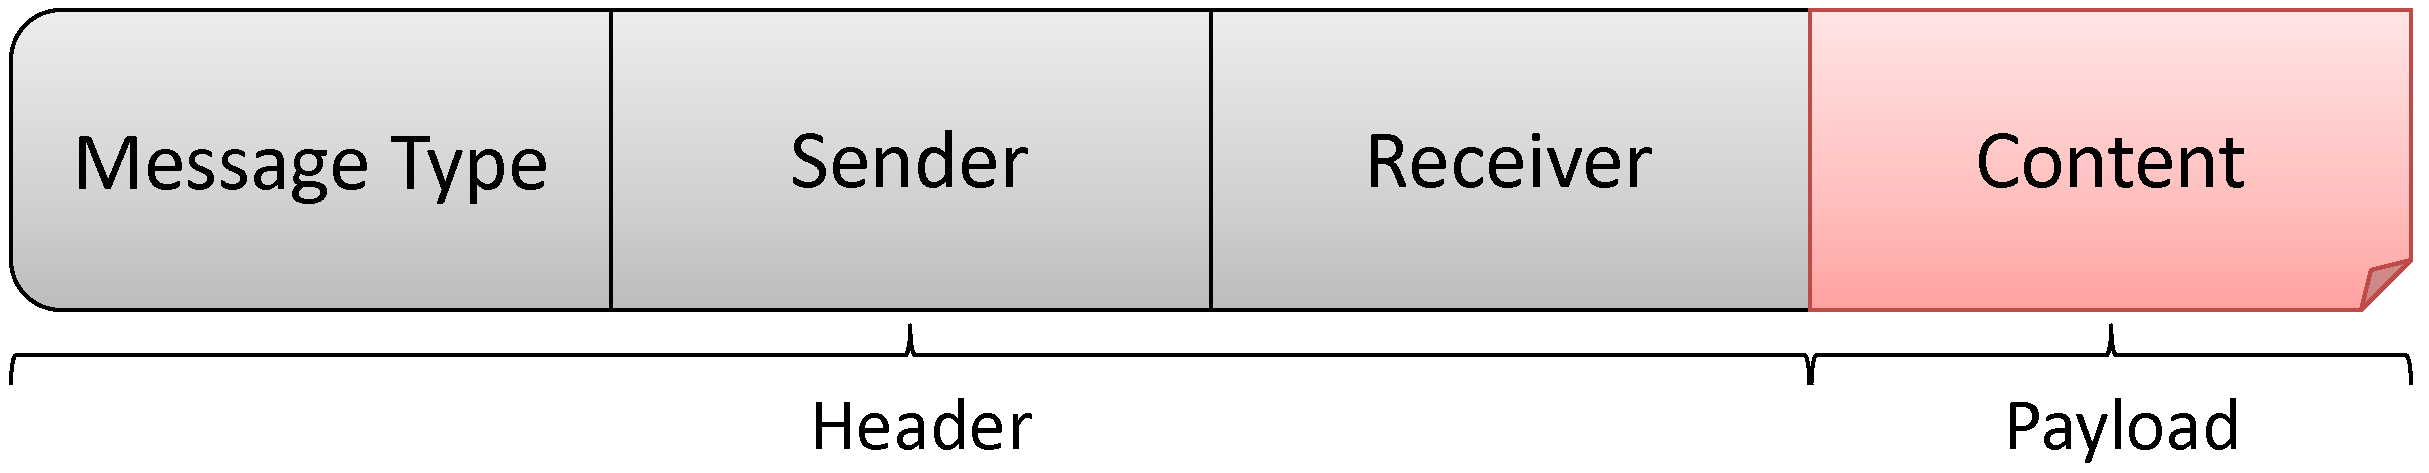
\includegraphics[width=0.7\linewidth]{img/Nachrichtenstruktur.png}
	\captionof{figure}[Nachrichtenstruktur]{Struktur einer Nachricht}
	\label{fig:Nachrichtenstruktur}
\end{minipage}
\vspace{0.5em}

Die einzelnen Teile einer Nachricht werden durch ein definiertes Trennzeichen separiert. Hierbei handelt es sich um ein nicht druckbares Zeichen, um den Zeichenraum der Nutzer beim Chatten nicht unnötig einzuschränken. Ein anderes ebenso nicht druckbares Zeichen zeigt das Ende dieser Nachricht an.

Während Bestandteile des Headers nicht mehr weiter unterteilbar sind, wird der Inhalt je nach Nachrichtentyp noch feiner strukturiert, indem in ihm das gleiche Trennzeichen wiederholt zur Anwendung kommt.

Der Nachrichtentyp wird durch die Definition eines Aufzählungstypen mit 13 zu unterscheidenden Werten realisiert. Das Absender-Feld hält den Namen des Benutzers als Zeichenkette fest, wohingegen das Empfänger-Feld einen Chatraum als positive Ganzzahl kodiert. Dies hat den Grund, dass zur Kommunikation immer ein Chatraum erforderlich ist. Alle Nachrichten werden zunächst als Broadcast gehandhabt, allerdings kann durch einen Chatraum von zwei Nutzern Unicast-Kommunikation verwirklicht werden. 
%TODO ist vielleicht zu system nah? das Protokoll ist ja eher auf einer abstrakten Schicht. Und steht mehr oder weniger unten nochmal

Bei diesem Vorgehen nimmt der Standard-Chatraum mit der Nummer \textit{0} eine besondere Rolle ein. Jeder nicht verbundene Client befindet sich in einem individuellen Standard-Chatraum mit dem Server. Er ist die Anlaufstelle für eingehende Verbindungsanfragen, da erst im folgenden Schritt dem anfragenden Client dynamisch ein einzelner Chatraum zur Kommunikation mit dem Server zugewiesen werden kann. Nach dem Verbindungsaufbau verfügt demnach jeder Client über einen eigenen Server-Chatraum und ggf. wenn er die Kommunikation mit anderen Clients sucht, über jeweils einen Chatraum für jeden Kommunikationspartner. Diese werden zunächst als Einzelchats zwischen zwei Nutzern erzeugt, können aber durch Benutzerinteraktion um beliebig viele Teilnehmer erweitert werden, wodurch Gruppenkommunikation möglich ist.

Das Protokoll lässt sich um beliebig viele weitere Funktionen erweitern. Hierzu muss nur ein neuer Nachrichtentyp eingeführt und die Kontrollstrukturen des Clients und Servers angepasst werden.

\subsubsection{Registrierung}
Ein Client meldet sich als ein Benutzer beim Server an. Dieser muss zuvor über eine Registrierung mit frei wählbarem Benutzernamen und Passwort angelegt.

Hierzu schreibt das Protokoll folgendes Verhalten vor: 
Der Client sendet eine Registrierungsanfrage an den Server. Diese ist vom Nachrichtentyp \textit{register} und trägt im Absender-Feld den gewünschten Benutzernamen. Als Receiver wird der Standard-Chatraum des Servers angegeben. Der Inhalt der Nachricht ist das verschlüsselt zu übertragende Passwort des Benutzers.

\vspace{1em}
\begin{minipage}{\linewidth}
	\centering
	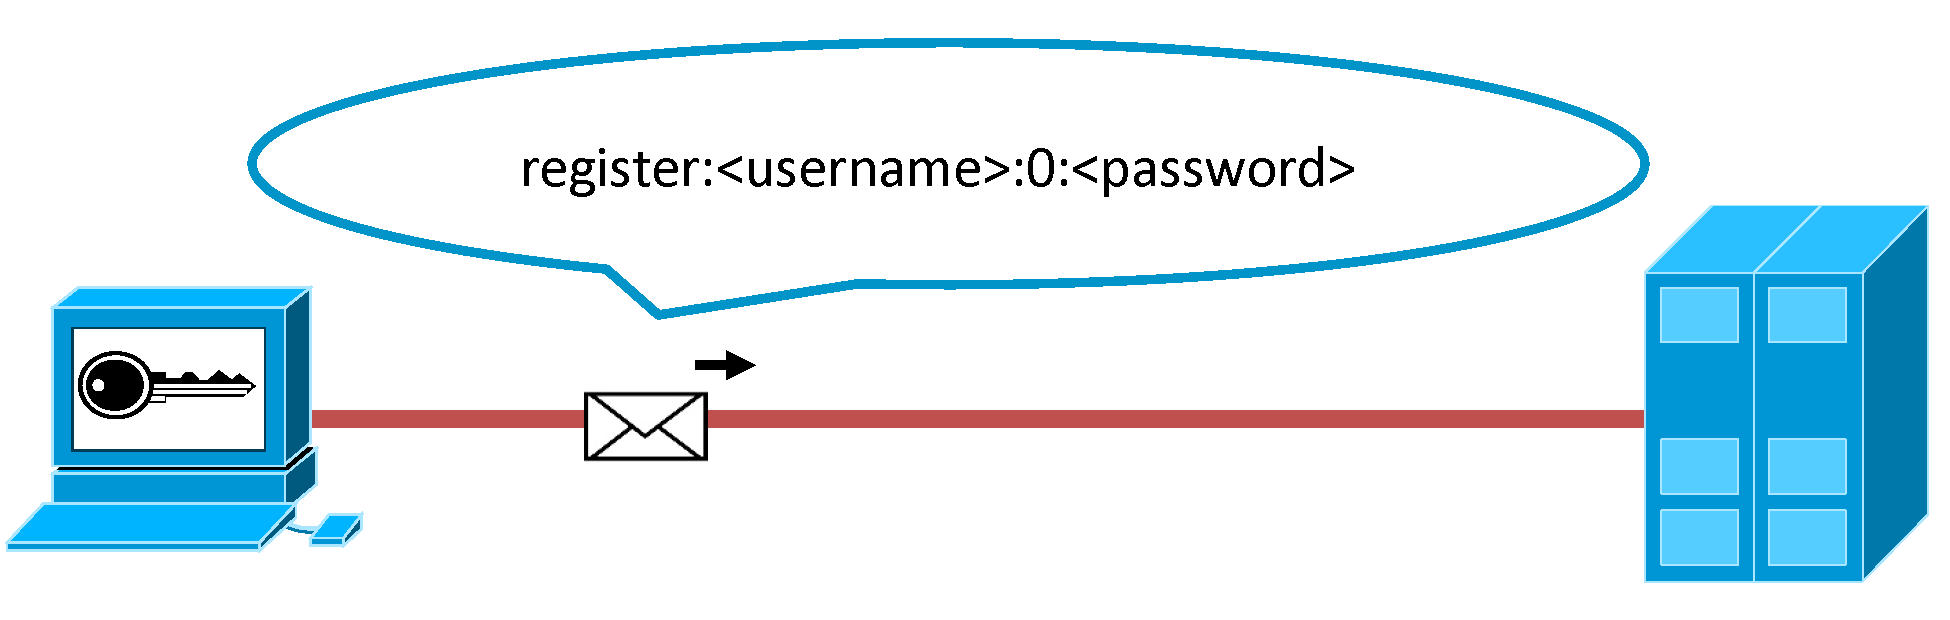
\includegraphics[width=0.7\linewidth]{img/register1.png}
	\label{fig:Registrierung1}
\end{minipage}
\vspace{0.5em}

Wenn der Server die Nachricht empfängt, quittiert er den Erfolgsfall, indem ebenfalls eine  \textit{register}-Nachricht, mit dem Inhalt \glqq ok\grqq{} zurückgeschickt wird. Sollte der Benutzername bereits verwendet werden, wird eine \textit{refused}-Nachricht mit Inhalt \glqq registration failed, name in use\grqq{} versendet.

\vspace{1em}
\begin{minipage}{\linewidth}
	\centering
	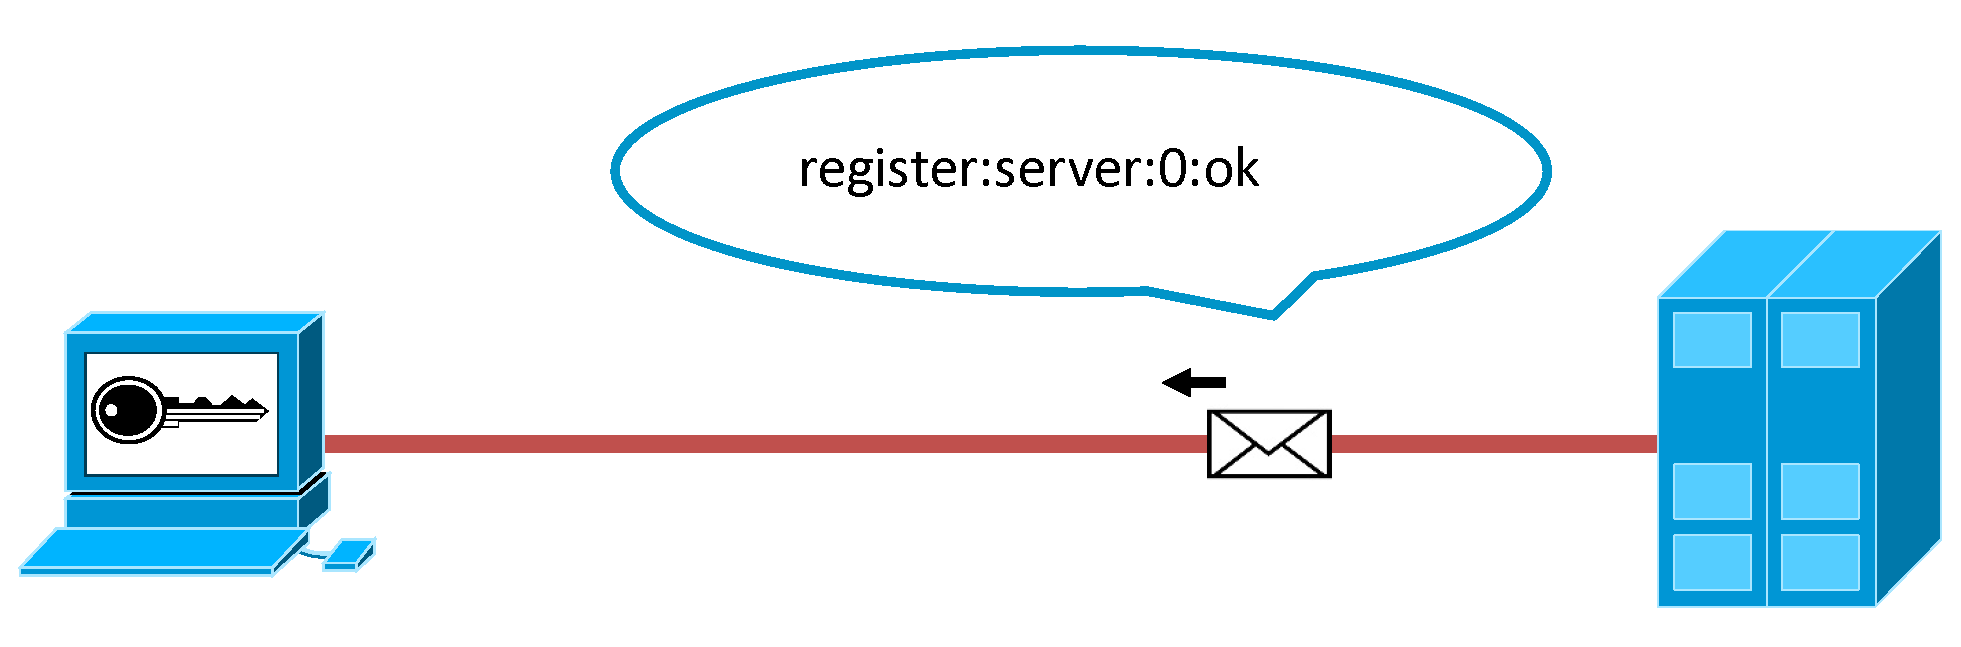
\includegraphics[width=0.7\linewidth]{img/register2.png}
	\label{fig:Registrierung2}
\end{minipage}
\vspace{0.5em}

\subsubsection{Einloggen}
Sobald ein Benutzer registriert wurde, kann sich der Client nun unter Angabe des Benutzernamens und Passworts beim Server per \textit{connect}-Nachricht einloggen. Da noch kein Chat zu diesem existiert, wird der Standard-Chatraum adressiert.

\vspace{1em}
\begin{minipage}{\linewidth}
	\centering
	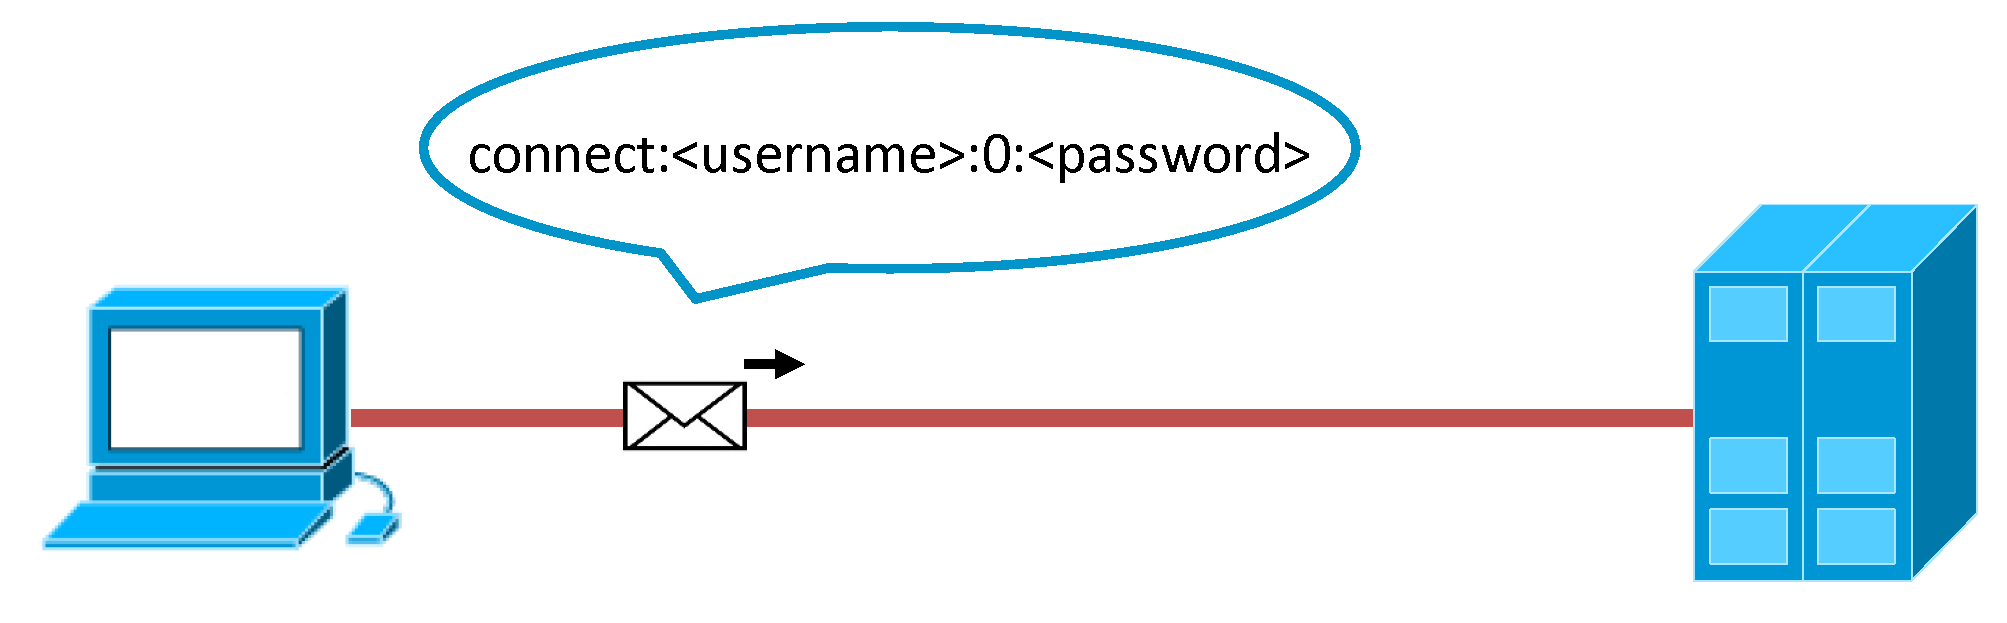
\includegraphics[width=0.7\linewidth]{img/connect1.png}
	\label{fig:connect1}
\end{minipage}
\vspace{0.5em} 

Der Verbindungsversuch hat zwei mögliche Resultate:
\begin{itemize}
	\item \textbf{Einloggen erfolgreich}
	
	In diesem Fall antwortet der Server ebenfalls mit einer \textit{connect}-Nachricht. Die Empfänger-Nummer stellt die ID des Chatraums dar, indem dieser Client zukünftig mit dem Server kommuniziert, künftig Server-Chatraum genannt. Das erfolgreiche Verbinden wird zusätzlich durch ein \glqq ok\grqq{} im Inhalt der Nachricht ausgedrückt.
	\item \textbf{Einloggen fehlgeschlagen}
	
	Sollte das Verbinden nicht gelingen, wird vom Server eine an den Standard-Chatraum adressierte \textit{refused}-Nachricht versendet, deren Inhalt Aufschluss über die Hintergründe des Misserfolgs liefert. Hierfür existieren vier verschiedene Szenarien.
	\begin{enumerate}
		\item \textbf{der Benutzer ist unbekannt} \newline
			Wird ein Benutzername übergeben, welcher dem Server nicht bekannt ist, schlägt das Einloggen fehl. Der Inhalt der Nachricht lautet dann \glqq user not found in database\grqq{}. 	
		\item \textbf{das Passwort ist nicht korrekt} \newline
			Sollte das übergebene Passwort nicht mit dem in der Datenbank des Servers hinterlegtem Passwort des Benutzers übereinstimmen, kann der Client nicht eingeloggt werden. Der Inhalt der Nachricht lautet dann \glqq invalid password\grqq{}.
		\item \textbf{der angegebene Benutzer ist schon eingeloggt} \newline
			Hier ist bereits ein Benutzer mit dem angegebenen Benutzernamen mit dem Server eingeloggt. Der Inhalt der Nachricht lautet dann \glqq user already logged in\grqq.
		\item \textbf{der Client ist bereits eingeloggt} \newline
		    Wenn der Client sich bereits als ein Benutzer zum Server verbunden hat, lehnt der Server ein erneutes Einloggen ab. Der Inhalt der Nachricht lautet dann \glqq you are already logged in to an account\grqq.
	\end{enumerate}
	
		\vspace{1em}
		\begin{minipage}{\linewidth}
			\centering
			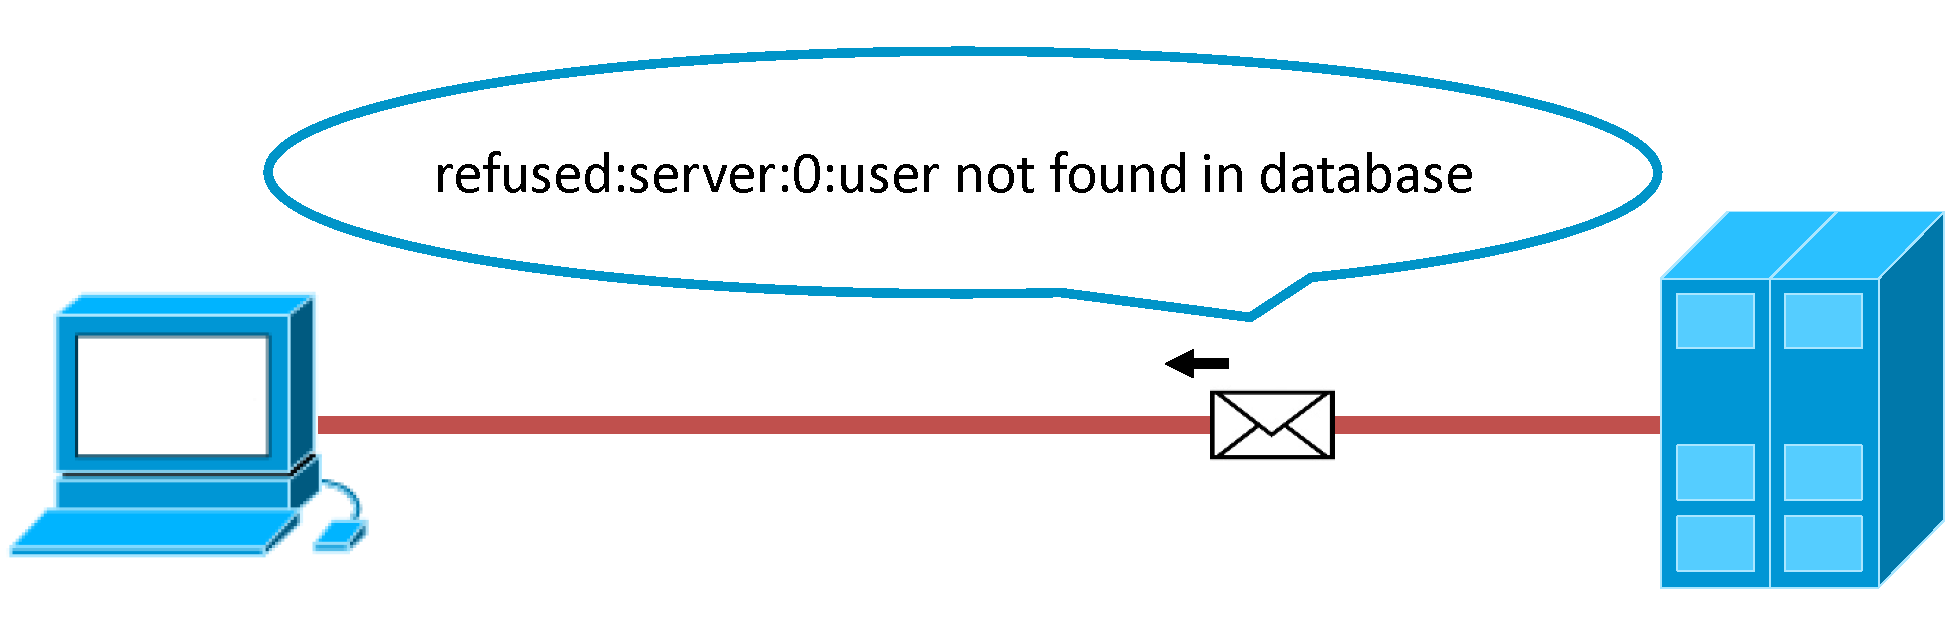
\includegraphics[width=0.7\linewidth]{img/connect2.png}
			\label{fig:connect2}
		\end{minipage}
	
\end{itemize}

\subsubsection{Kontaktanfrage}
Sobald der Client eingeloggt ist, kann er nun mit Kontakten chatten. Kontakte sind beidseitig, das heißt, man kann nicht mit einem Benutzer befreundet sein, ohne gleichzeitig auch Kontakt des Benutzers zu sein.

Diese Kontakte müssen vor dem Chatten angelegt werden. Eine \textit{addcontact}-Nachricht, adressiert an den Server, teilt diesem mit, dass dem im Inhalt der Nachricht genannten Benutzer eine Kontaktanfrage gestellt werden soll.

\vspace{1em}
\begin{minipage}{\linewidth}
	\centering
	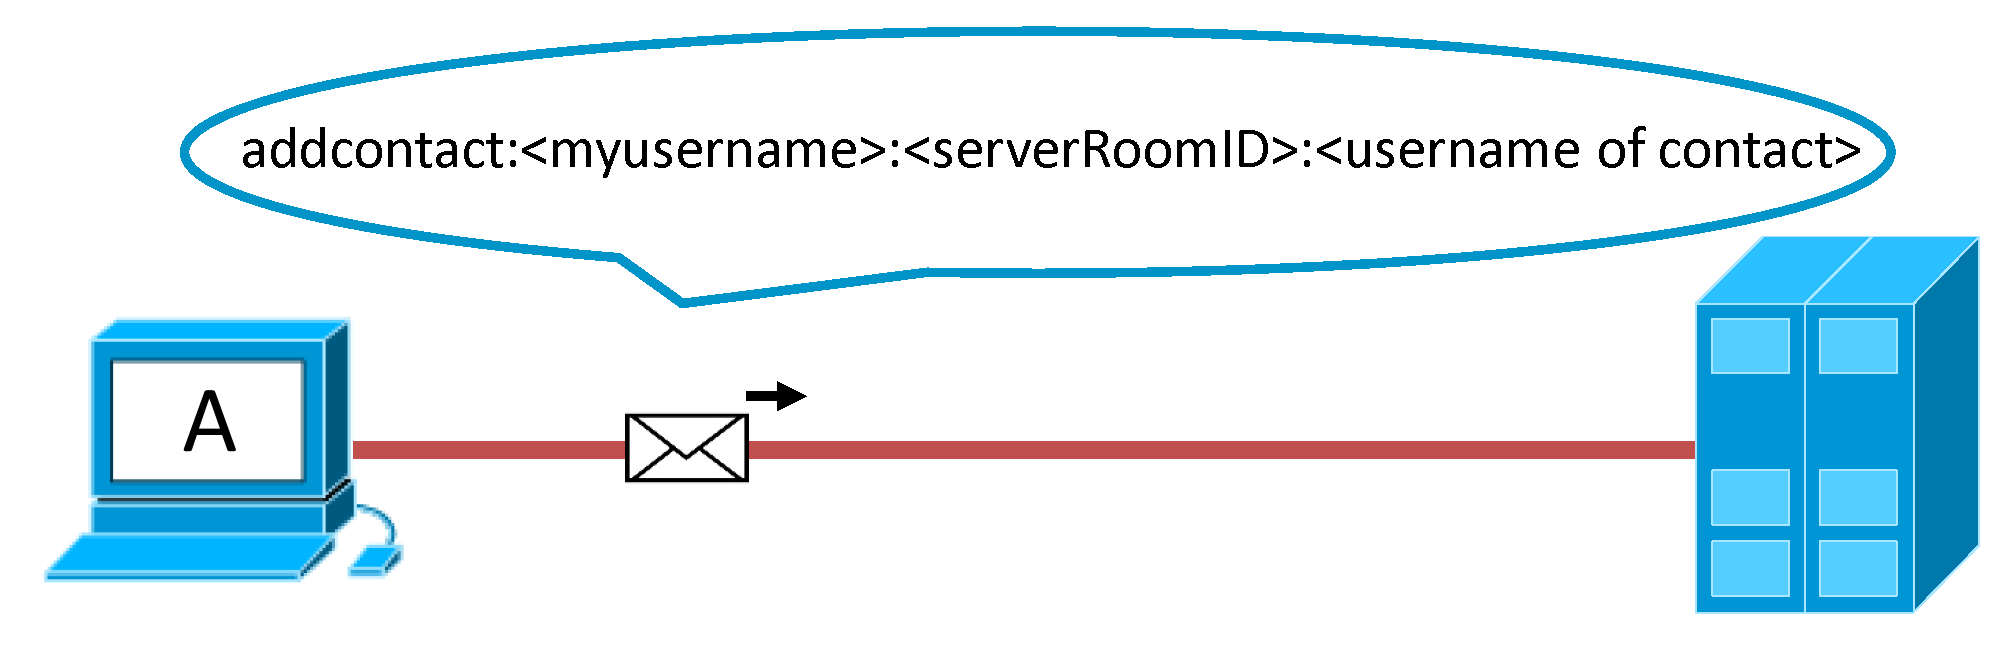
\includegraphics[width=0.7\linewidth]{img/addcontact1.png}
	\label{fig:addcontact1}
\end{minipage}
\vspace{0.5em} 

Der Server gibt diese Intention dem requestierten Benutzer weiter, sollte dieser eingeloggt sein.

\vspace{1em}
\begin{minipage}{\linewidth}
	\centering
	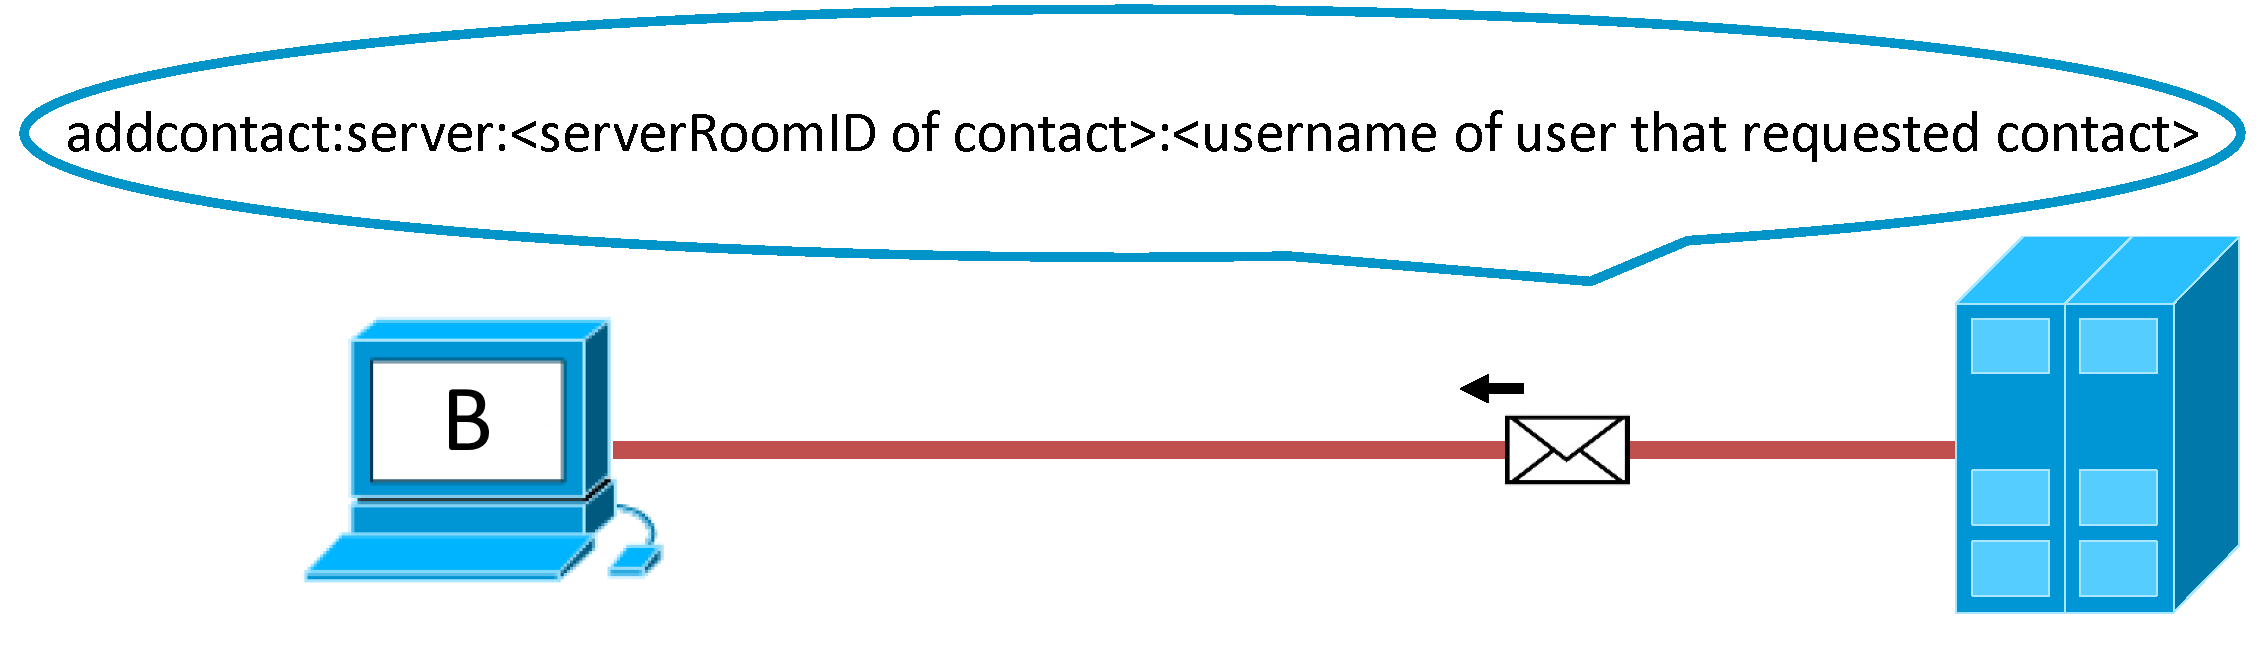
\includegraphics[width=0.7\linewidth]{img/addcontact2.png}
	\label{fig:addcontact2}
\end{minipage}
\vspace{0.5em}

Eine Kontaktanfrage kann angenommen werden, indem man dem anfragenden User eine Kontaktanfrage zurück stellt.

Um eine Kontaktanfrage abzulehnen, kann eine \textit{remcontact}-Nachricht an den Server gesendet werden. Als Inhalt ist der Benutzernamen des anfragenden Benutzers zu nennen.

\vspace{1em}
\begin{minipage}{\linewidth}
	\centering
	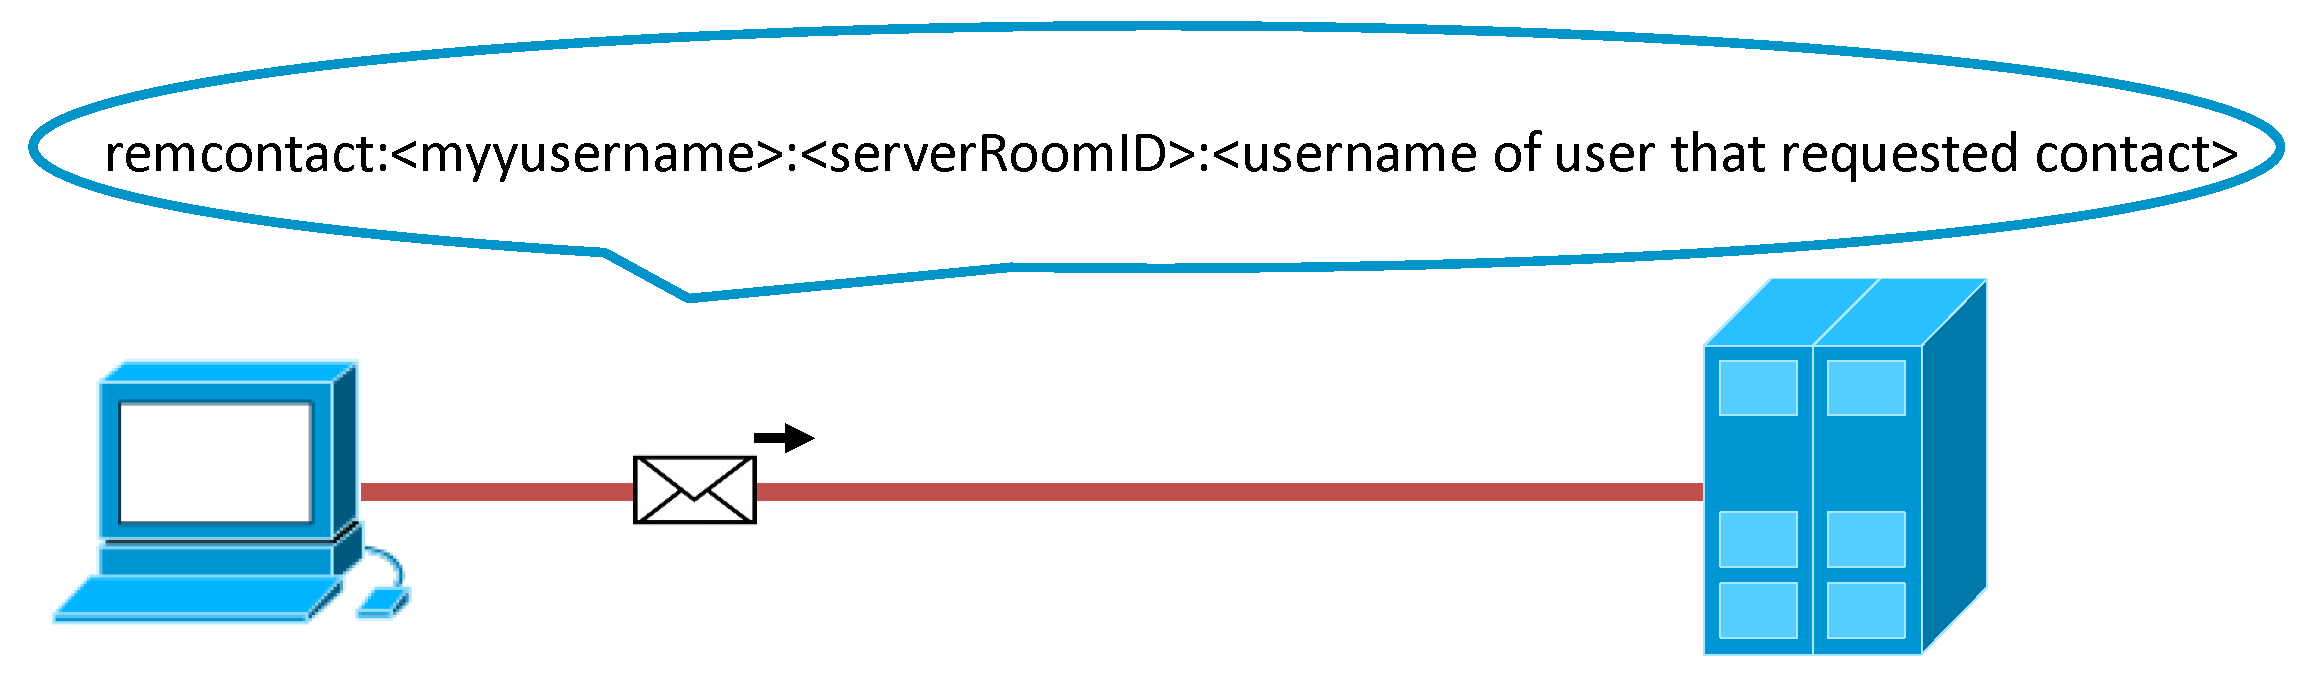
\includegraphics[width=0.7\linewidth]{img/remcontact1.png}
	\label{fig:remcontact1}
\end{minipage}
\vspace{0.5em} 

Über eine Nachricht in dieser Form kann auch ein Kontakt entfernt werden. Dies quittiert der Server mit einer \textit{remcontact}-Nachricht, welche den Benutzernamen des entfernten Kontakts als Inhalt trägt. Eine analoge Nachricht wird auch den an entfernten Kontakt gesendet.

Sollte der Client versuchen, einen Benutzer von seiner Kontaktliste zu entfernen, welcher sich nicht auf dieser befindet, oder versuchen, eine Kontaktanfrage von einem Benutzer abzulehnen, welcher keine Anfrage gestellt hat, wird die \textit{remcontact}-Nachricht vom Server mit einer \textit{refused}-Nachricht beantwortet und keine weiteren Aktionen ausgelöst. Der Inhalt der Nachricht lautet dann dementsprechend der Situation \glqq there is no contact request from \grq\textless{}username\textgreater\grq \grqq{} beziehungsweise \glqq there is no contact with name \grq\textless{}username\textgreater\grq \grqq{}.

\vspace{1em}
\begin{minipage}{\linewidth}
	\centering
	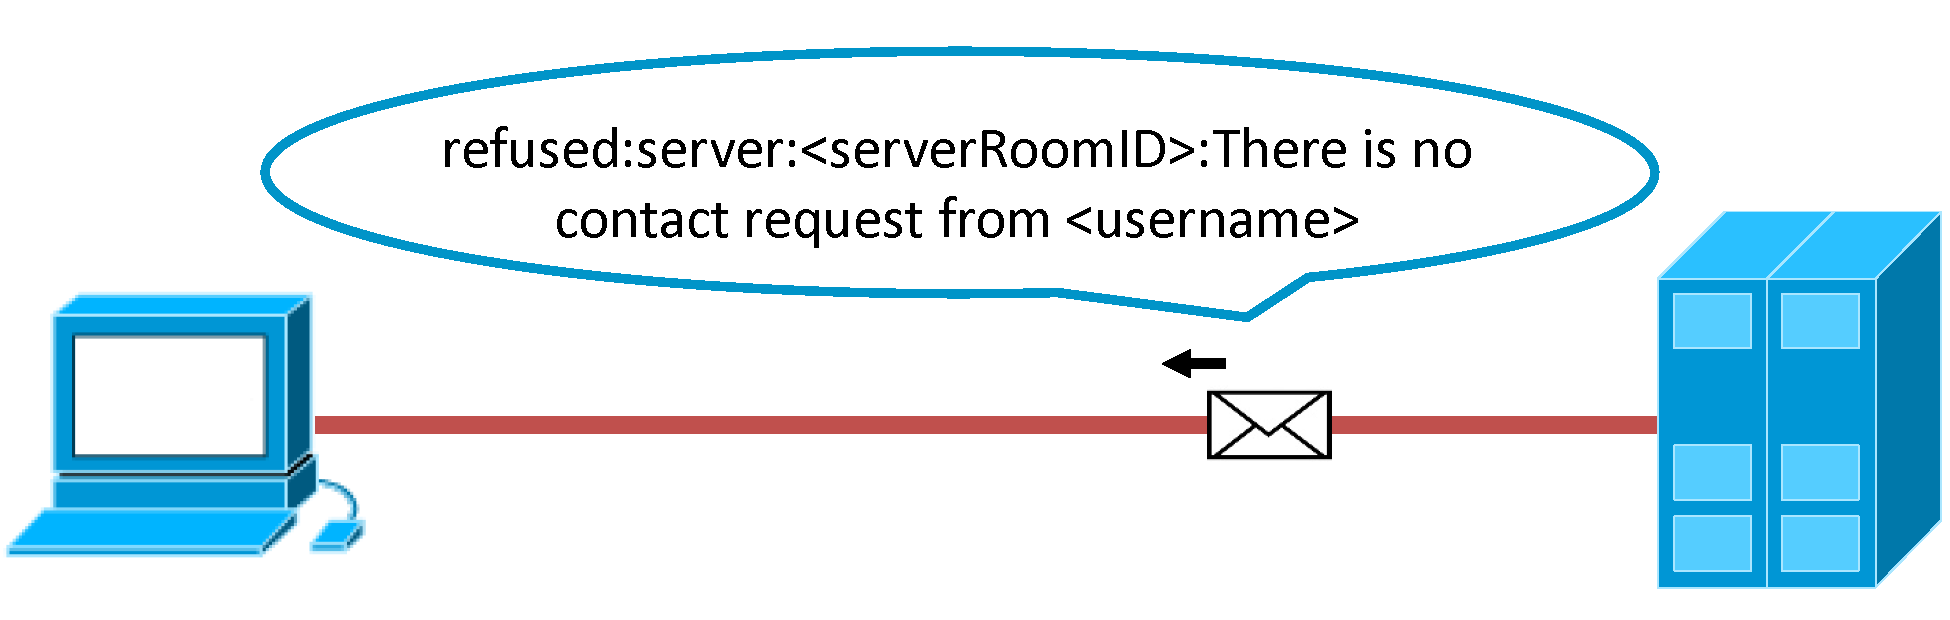
\includegraphics[width=0.7\linewidth]{img/remcontact2.png}
	\label{fig:remcontact2}
\end{minipage}
\vspace{0.5em}

Sollte sich der Online-Status eines Kontaktes ändern, durch Ein-/Ausloggen oder nach dem er als neuer Kontakt hinzugefügt wurde, wird der neue Status dem Benutzer durch eine \textit{offline}- oder \textit{online}-Nachricht mitgeteilt.

\vspace{1em}
\begin{minipage}{\linewidth}
	\centering
	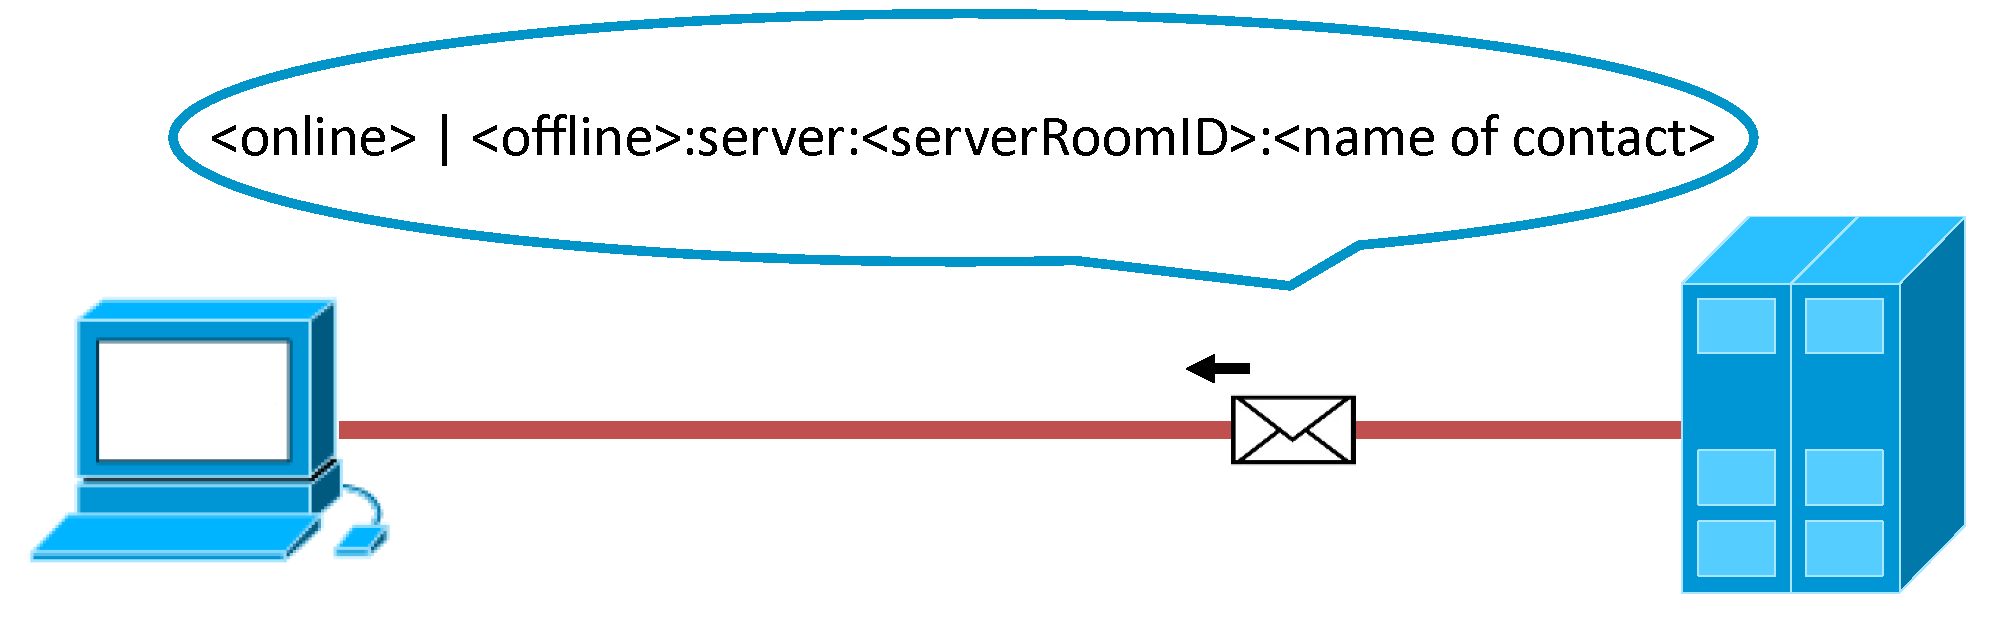
\includegraphics[width=0.7\linewidth]{img/status1.png}
	\label{fig:status1}
\end{minipage}

\subsubsection{Chatten}
Jeder Form des Chattens findet in einem Chatraum statt. Dieser muss zuerst vom Server erstellt werden. Hierzu muss der Client eine \textit{chatrequest}-Nachricht an den Server senden. Adressiert wird diese an den Serverchatraum, der Inhalt gibt an, mit welchem eingeloggten Kontakt man chatten möchte. Mit Benutzern, die nicht Kontakt des Clients sind, kann nicht gechattet werden.

\vspace{1em}
\begin{minipage}{\linewidth}
	\centering
	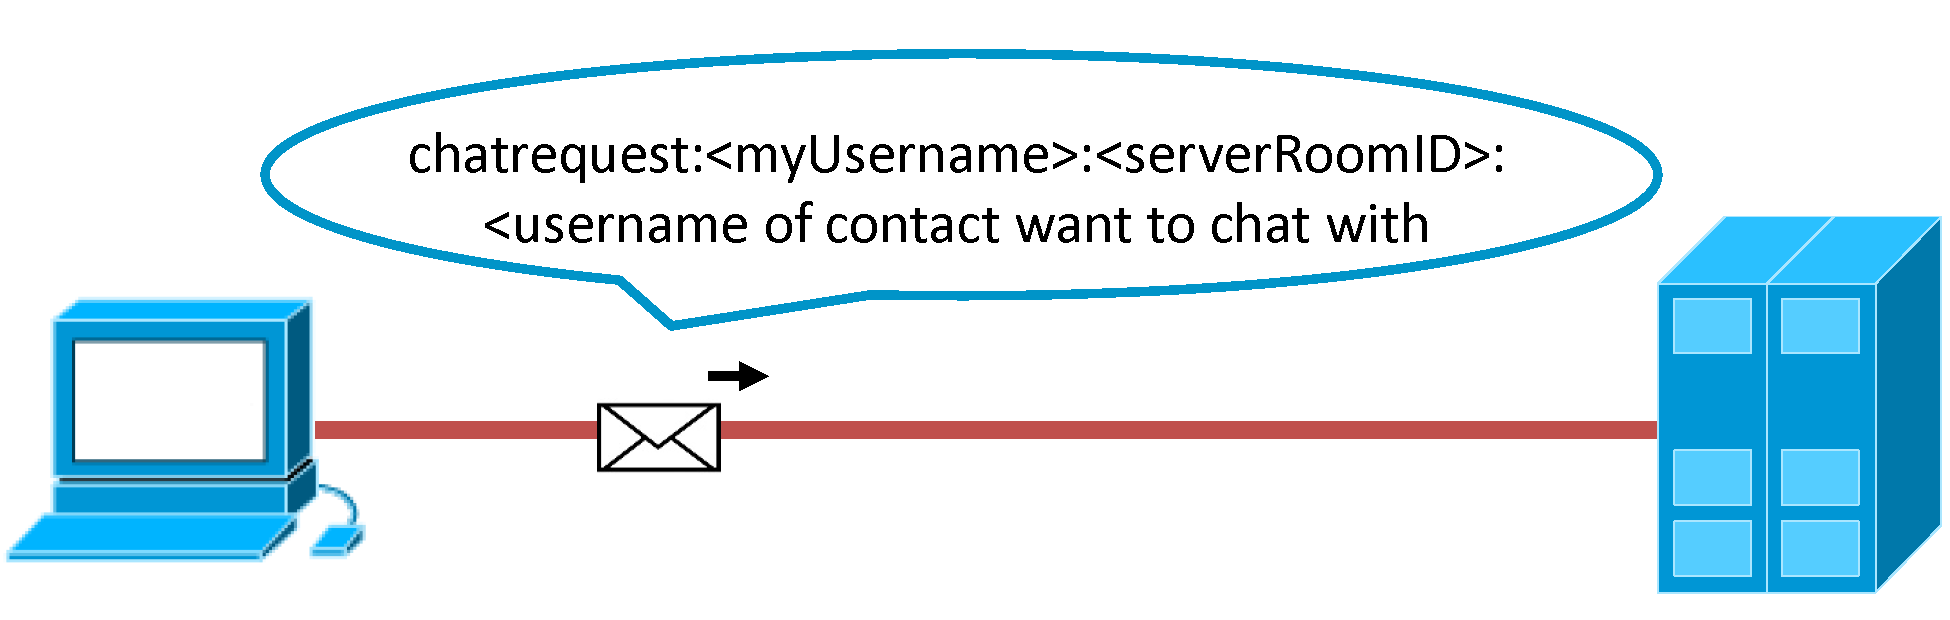
\includegraphics[width=0.7\linewidth]{img/chatrequest1.png}
	\label{fig:chatrequest1}
\end{minipage}
\vspace{0.5em}

Der Server verarbeitet die Anfrage, in dem er einen Chatraum mit einer einzigartigen ID erstellt und den anfragenden sowie den angefragten Benutzer zu dem Chatraum hinzufügt. Dem anfragenden Benutzer wird anschließend mit einer \textit{chatrequest}-Nachricht geantwortet, die als Empfänger-ID die Nummer des Chatraums trägt. Diese Nummer dient nun als Adresse aller \textit{chat}-Nachrichten, die in diesem Raum ausgetauscht werden. 

\vspace{1em}
\begin{minipage}{\linewidth}
	\centering
	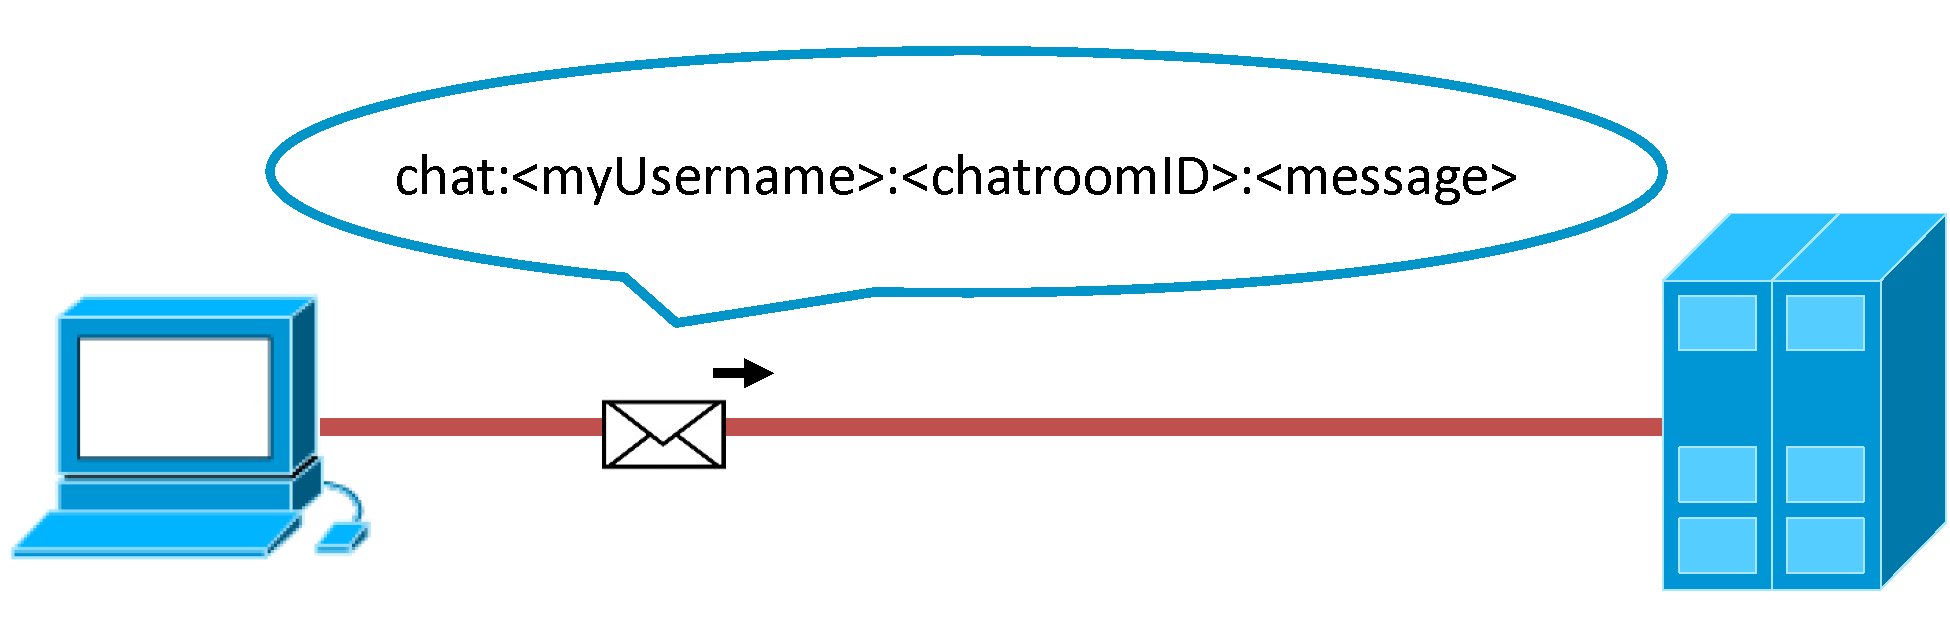
\includegraphics[width=0.7\linewidth]{img/chat1.png}
	\label{fig:chat1}
\end{minipage}
\vspace{0.5em}

Möchte der Benutzer einen weiteren Kontakt zu diesem Chat hinzufügen, sendet er eine analoge \textit{chatrequest}-Nachricht mit der Chatraum-ID als Empfänger-ID.

Ändert sich die Teilnehmerliste eines Chats, indem ein neuer Benutzer hinzugefügt wurde oder ein Benutzer den Chat verlässt, teilt der Server dies allen übrigen Teilnehmern im Chat mit einer \textit{userlist}-Nachricht mit. Im Inhalt dieser an den jeweiligen Chatraum adressierten Nachricht befinden sich die Benutzernamen aller Teilnehmer, durch das vom Protokoll genutzte Trennzeichen jeweils separiert.

\vspace{1em}
\begin{minipage}{\linewidth}
	\centering
	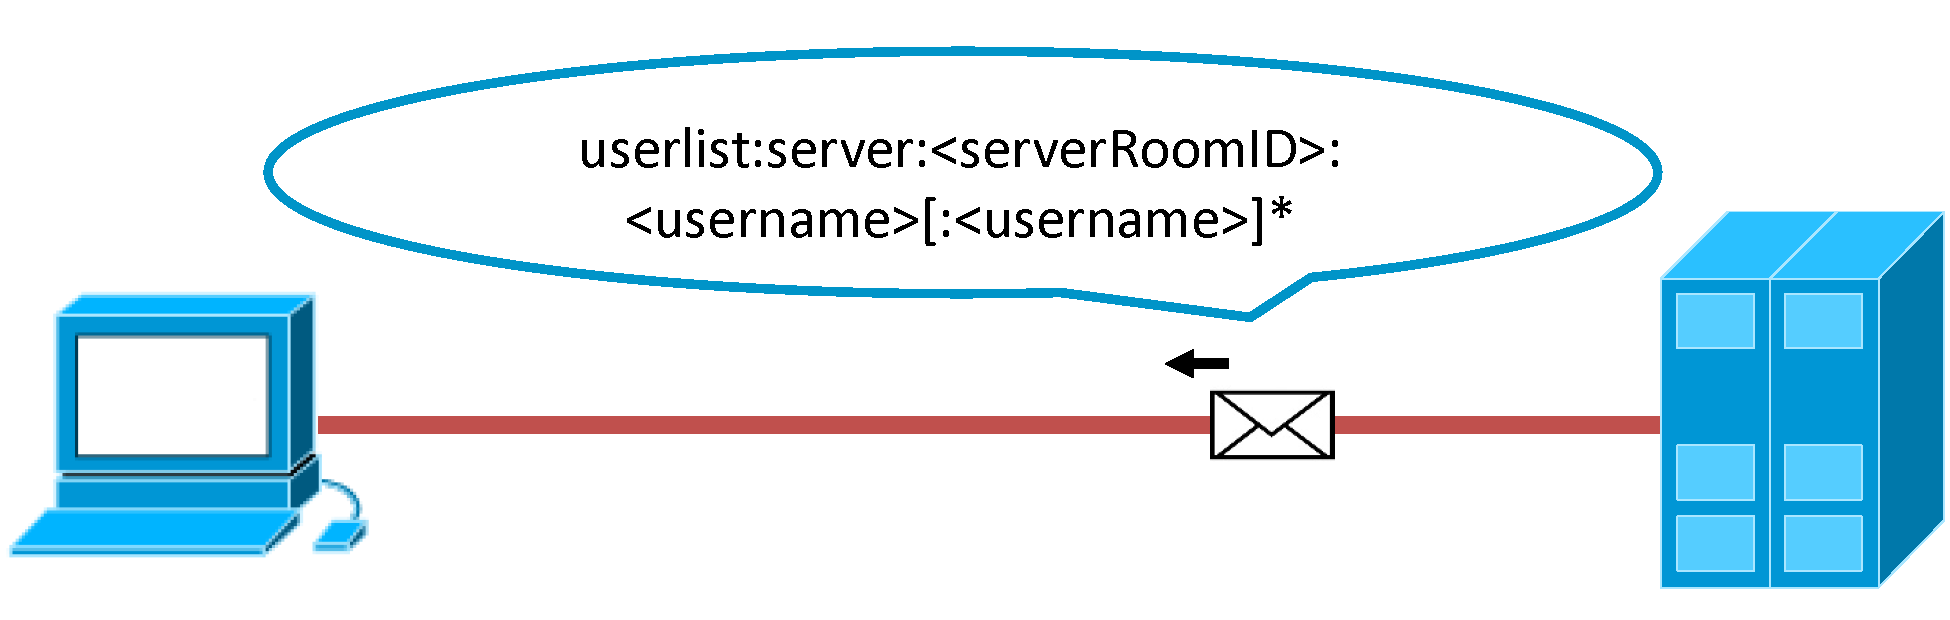
\includegraphics[width=0.7\linewidth]{img/userlist1.png}
	\label{fig:userlist1}
\end{minipage}
\vspace{0.5em}

Ein Chatraum wird durch Versenden einer an den jeweiligen Chatraum adressierte \textit{leavechat}-Nachricht verlassen. Dem Benutzer steht es offen einen Abschiedstext anzugeben, der nach dem Verlassen im Chat angegeben wird.

\vspace{1em}
\begin{minipage}{\linewidth}
	\centering
	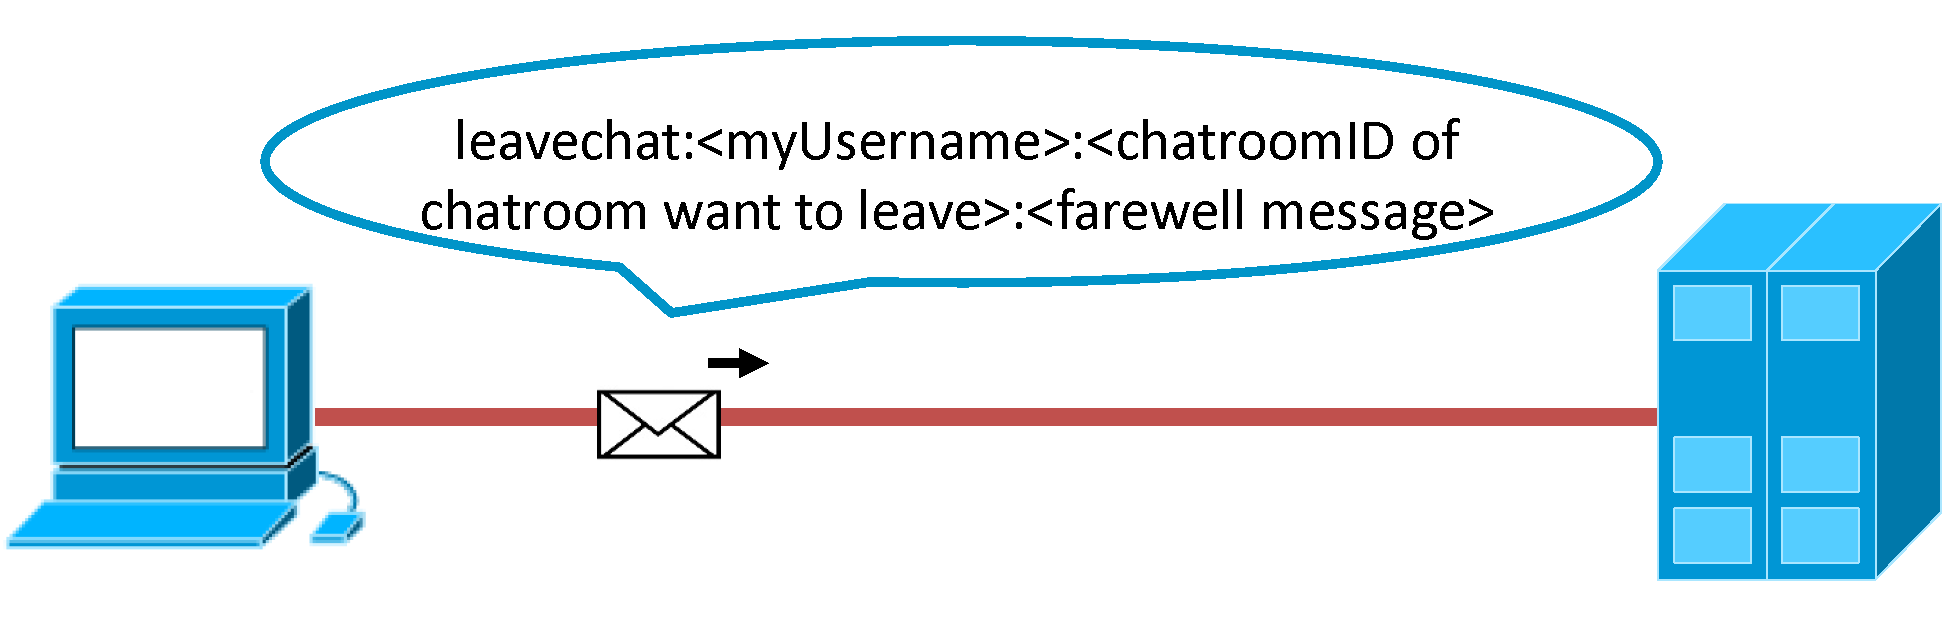
\includegraphics[width=0.7\linewidth]{img/leavechat1.png}
	\label{fig:leavechat1}
\end{minipage}
\vspace{0.5em}


\subsubsection{Ausloggen}
Das Ausloggen wird mit einer \textit{disconnect}-Nachricht bewerkstelligt. Wenn der Server diese durch eine weitere \textit{disconnect}-Nachricht dem Inhalt \glqq ok\grqq{}. bestätigt, wurde der Benutzer erfolgreich ausgeloggt.

\vspace{1em}
\begin{minipage}{\linewidth}
	\centering
	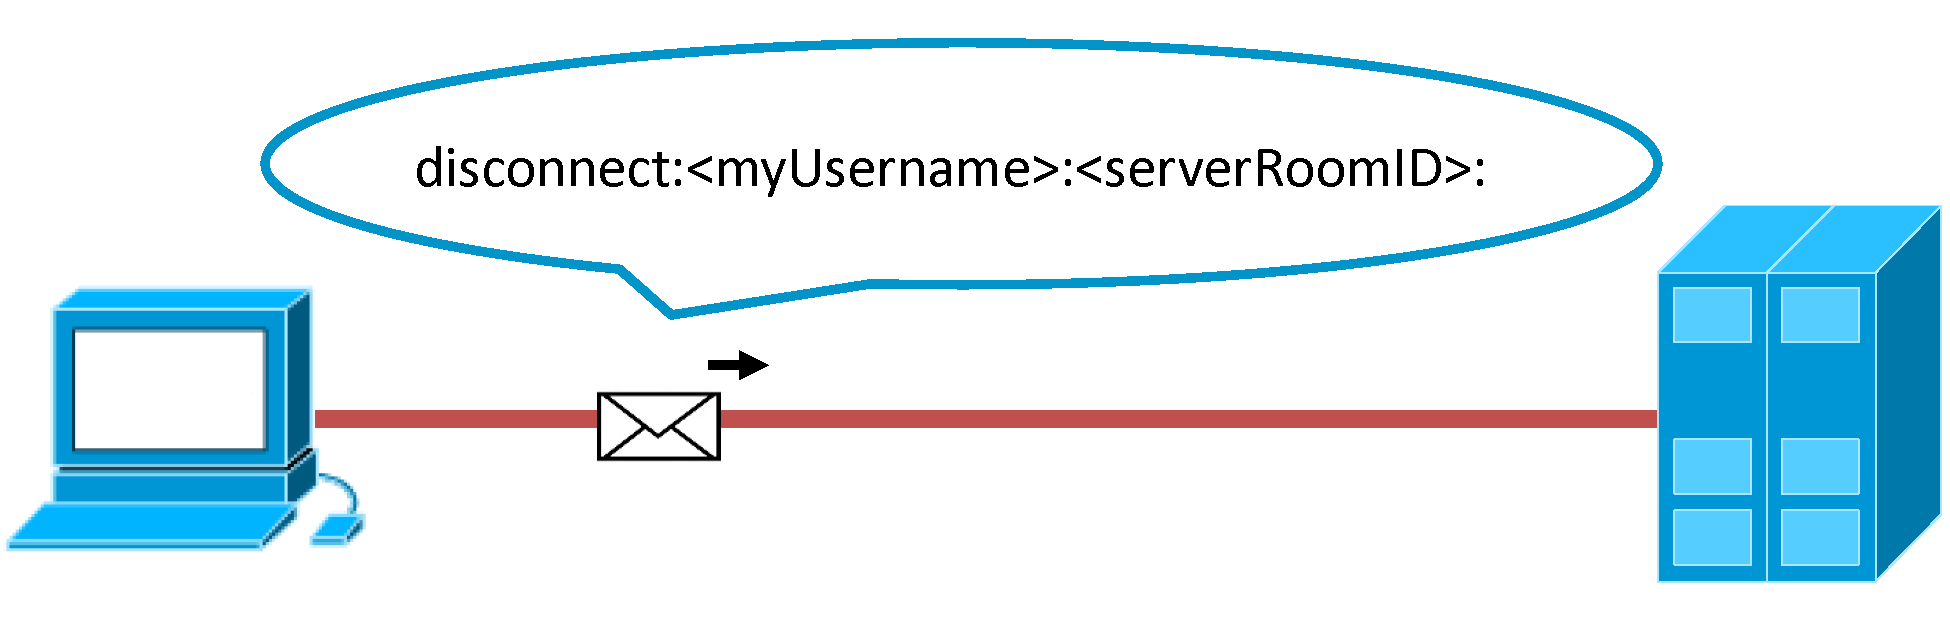
\includegraphics[width=0.7\linewidth]{img/disconnect.png}
	\label{fig:disconnect}
\end{minipage}


\subsection{Implementierungslogik}
In diesem Abschnitt soll beschrieben werden, wie das Programm von der Logik her arbeitet. Auf die konkreten Datenstrukturen, die zur Informationshaltung und -verwaltung genutzt werden wird nicht näher eingegangen. 

Während des Elaboration Tasks erzeugt und konfiguriert der Server seinen Kommunikationssocket für eingehende Verbindungsanfragen auf der Transportschicht. Hierzu zählt beispielsweise die Initialisierung von IP-Adresse und Port, sowie das Binden des Socket an diese. Daraufhin erzeugt und startet er einen weiteren Task, folgend Main-Task genannt. 

Der Main-Task hat die Aufgabe auf eingehende Verbindungsanfragen zu lauschen und eine Verbindung zwischen Client und Server auf der Transportschicht herzustellen. Zum Lauschen auf den Socket benutzt er eine blockierende Subroutine, die zurückkehrt, sobald Aktivität anliegt. Daraufhin erzeugt der Main-Task für diesen Client einen eigenen Socket und Task. Als letzte Aktion startet der Main-Task diesen Client-Task und fährt nach dessen Aktivierungsphase mit einem erneuten Lauschen auf den Server-Socket fort. Solch ein Client-Task wird für jeden Nutzer bzw. Client erzeugt. 

\vspace{1em}
\begin{minipage}{\linewidth}
	\centering
	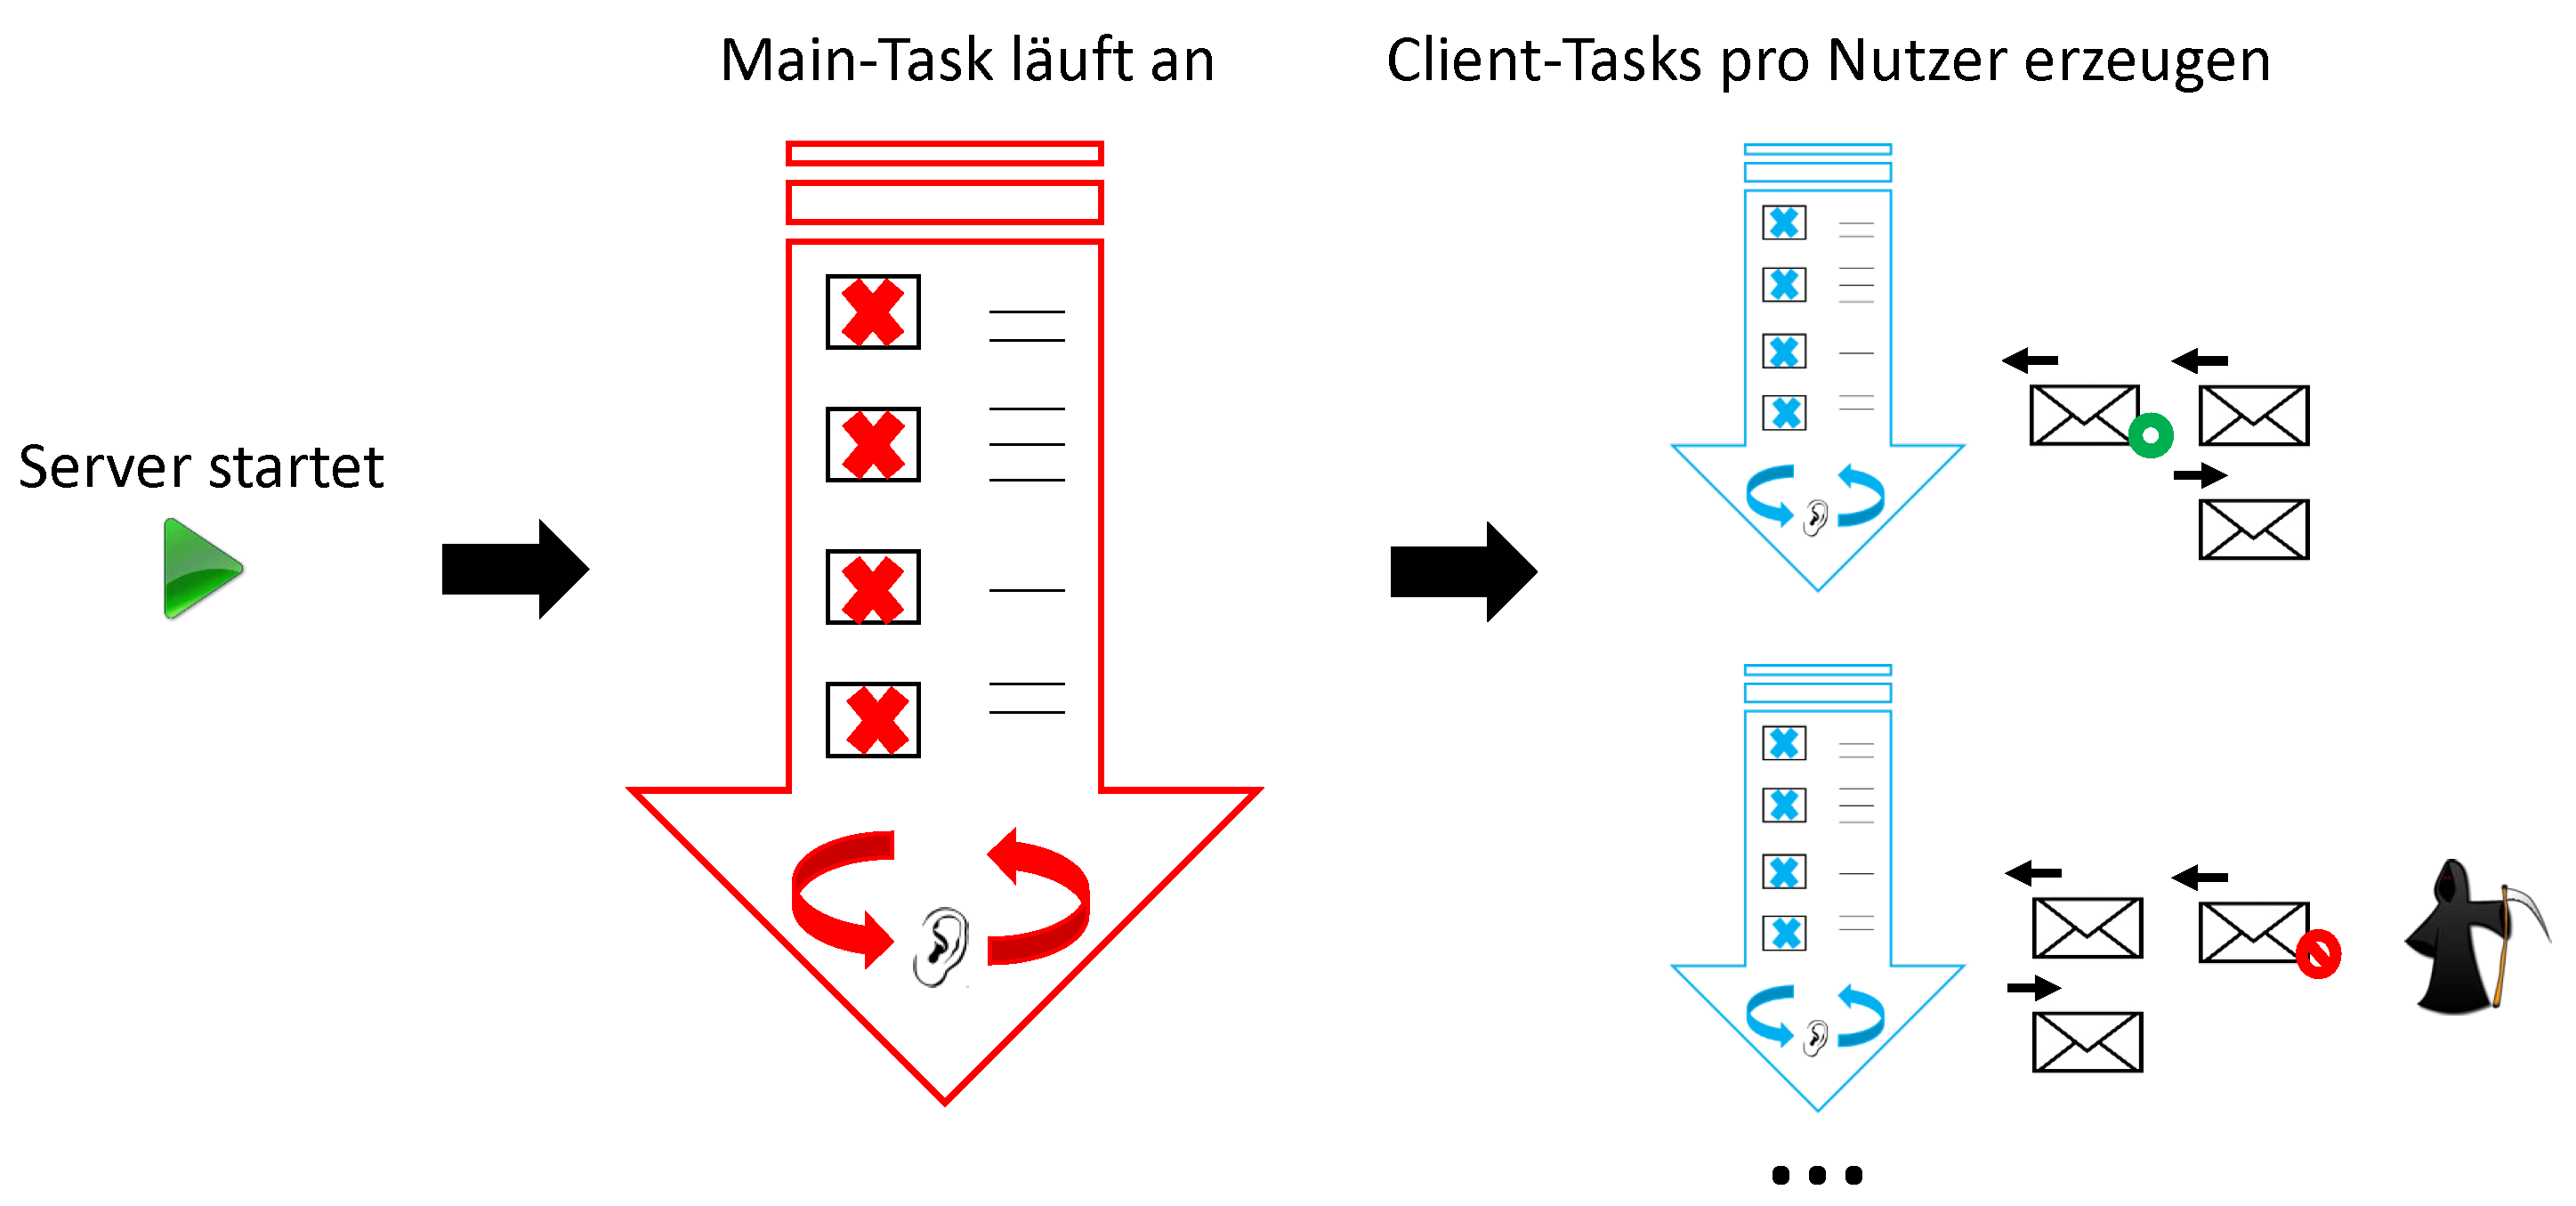
\includegraphics[width=1\linewidth]{img/Implementierungslogik.png}
	\label{fig:Implementierungslogik}
\end{minipage}
\vspace{0.5em}

Ein Client-Task setzt in seinen Handlungsroutinen das Kommunikationsprotokoll um. Dies bedeutet, dass er auf seinem Socket auf eingehende Nachrichten horcht und sobald solch eine eintrifft, je nach Nachrichtentyp handelt. Dies beinhaltet ebenso den vom Protokoll vorgesehenen Verbindungsaufbau auf der Anwendungsschicht mittels einer \textit{connect}-Nachricht. Analog zum Server kehrt er nach solch einer Routine zum erneuten Horchen zurück. Sobald der Wunsch auf Verbindungsabbau von einem der beiden Seiten gestellt wird, typischerweise vom Client, wird der Client-Task verschiedene Verwaltungsakte durchführen. Dies beinhaltet z.B. dass er den Client aus dessen Chaträumen entfernt und den Socket schließt. Ist dies alles vollbracht, endet der Client-Task. Bei erneutem Verbindungsaufbau des Nutzers legt der Main-Task einen frischen Client-Task an, welcher analog verfährt.

Die Clientseite des Chatprogramms arbeitet sehr ähnlich. Da diese aber zu jedem Zeitpunkt nur auf einen Socket lauschen muss, wird nur ein Task zum Abfragen der Socketverbindung verwendet, der Main-Task entfällt.

\vspace{1em}
\begin{minipage}{\linewidth}
	\centering
	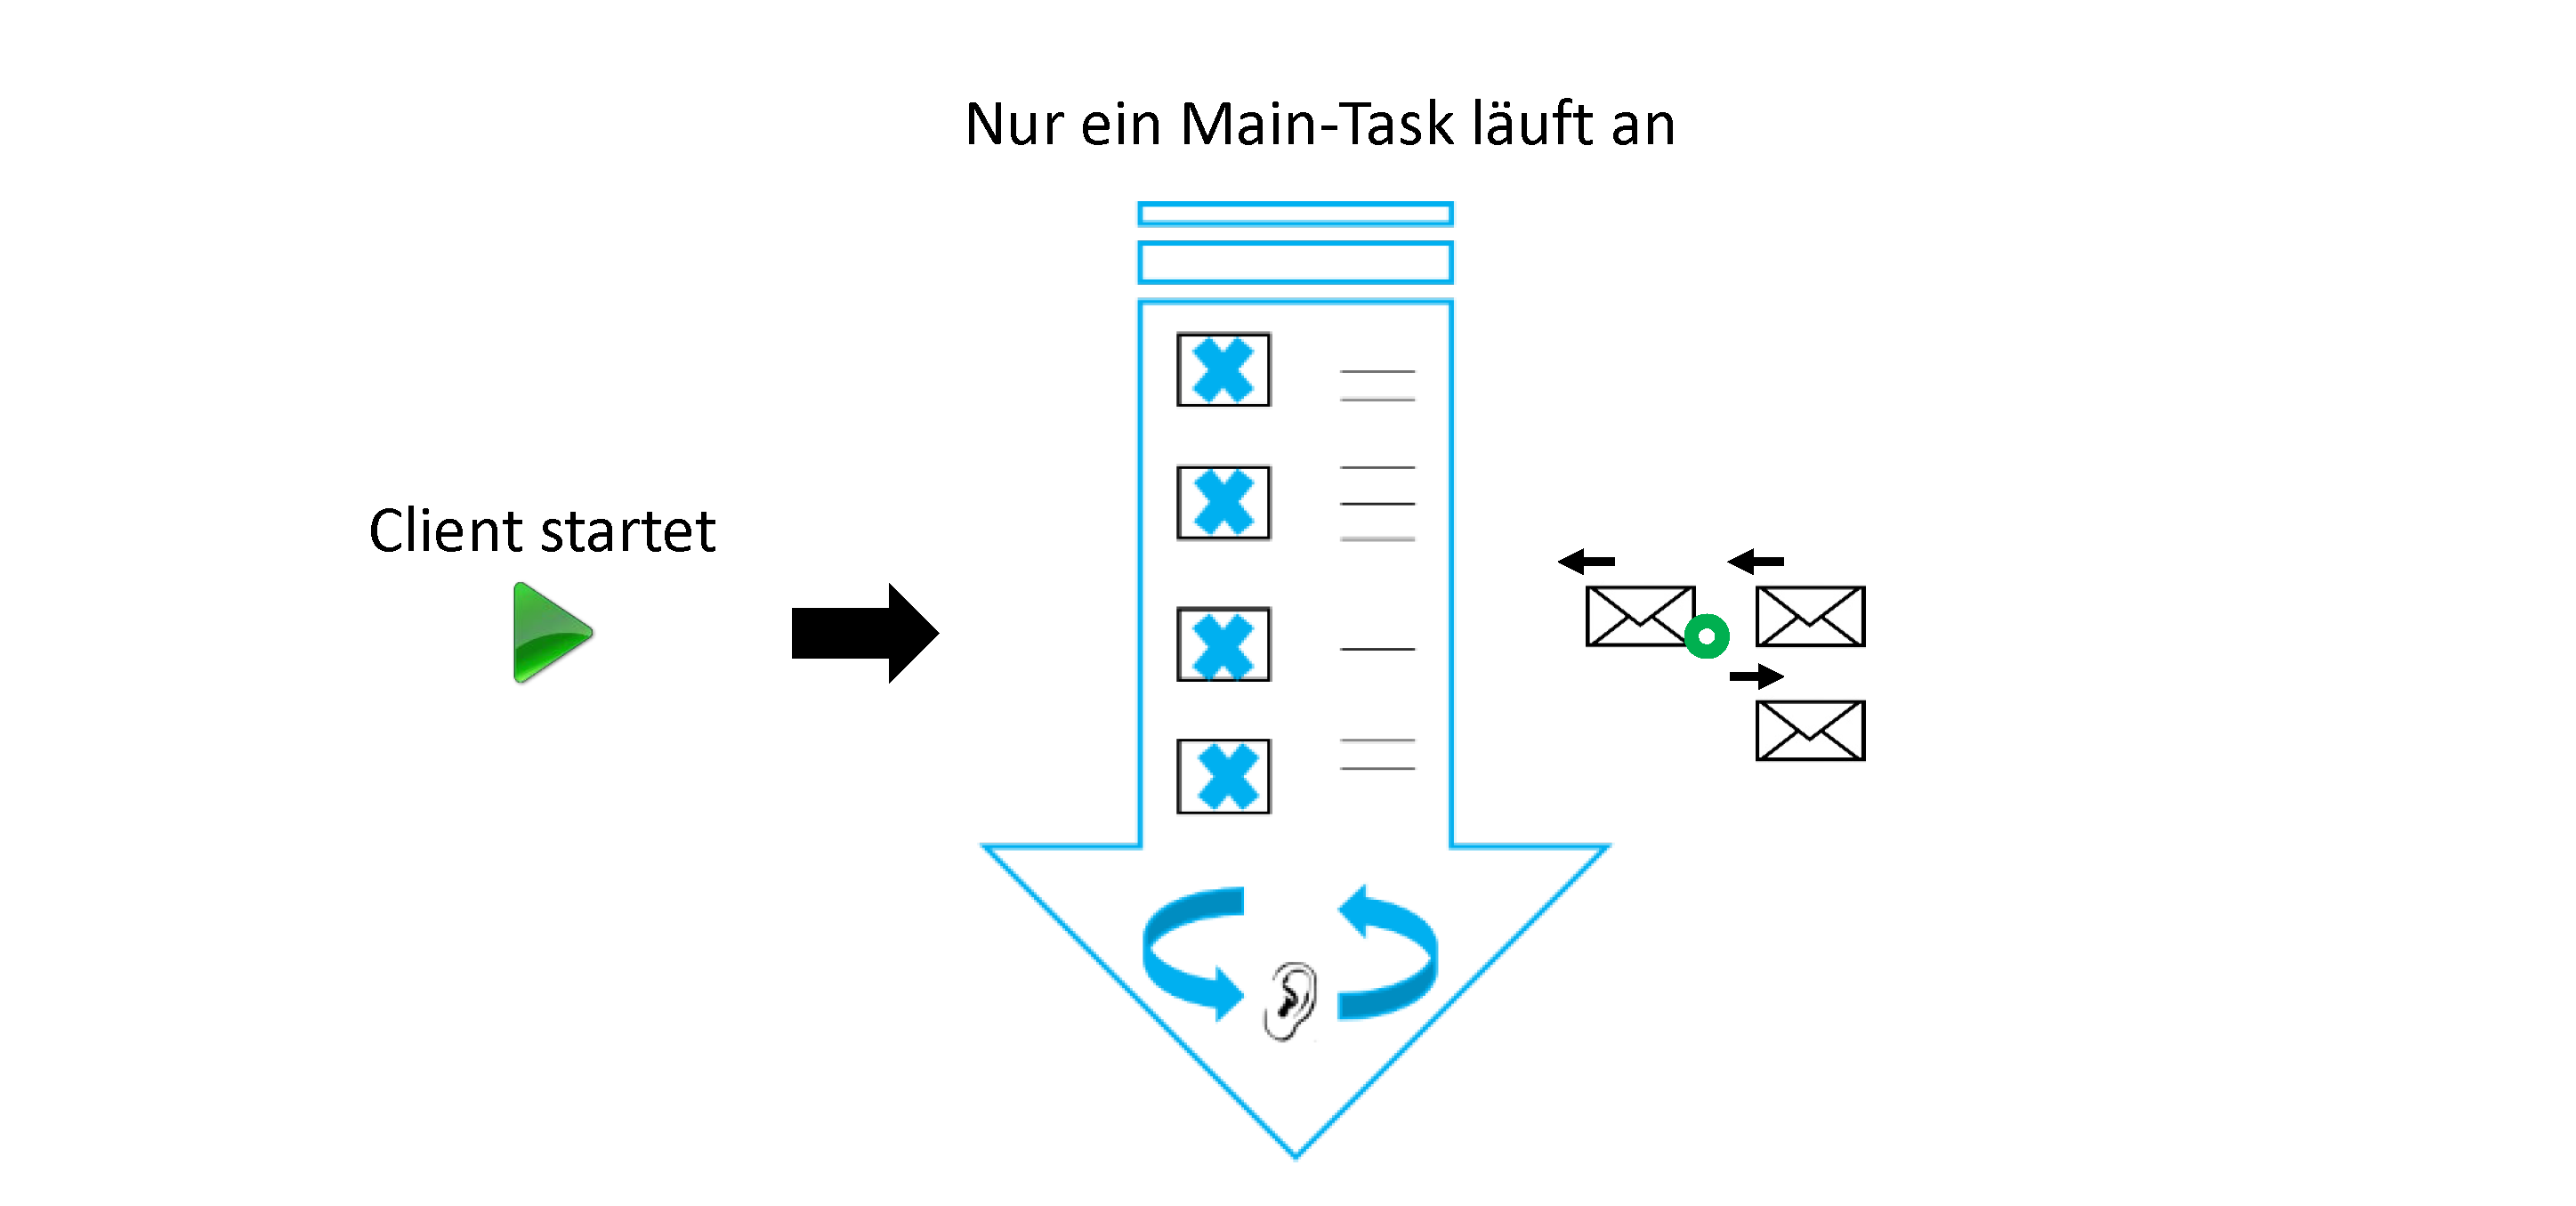
\includegraphics[width=1\linewidth]{img/Implementierungslogik2.png}
	\label{fig:Implementierungslogik Client}
\end{minipage}
\vspace{0.5em}

\subsection{Klassendiagramme}
Die Klassendiagramme können aufgrund ihrer Größe dem beigelegten Verzeichnis 
\glqq Klassendiagramme\grqq{} entnommen werden.

% ----------------------------------------------------------------------------------------------------------
% Probleme
% ----------------------------------------------------------------------------------------------------------

\newpage
\section{Benutzerhandbuch}
Im Folgenden soll die Benutzung der Oberflächen erklärt werden, um dem Benutzer einen leichten Einstieg zu gewähren.
\subsection{Server}
Die Server-GUI dient als Oberfläche dazu, die Steuerung der Serverlogik einfach zu gestalten und somit eine effiziente Verwaltung zu gewährleisten.

\vspace{1em}
\begin{minipage}{\linewidth}
	\centering
	\frame{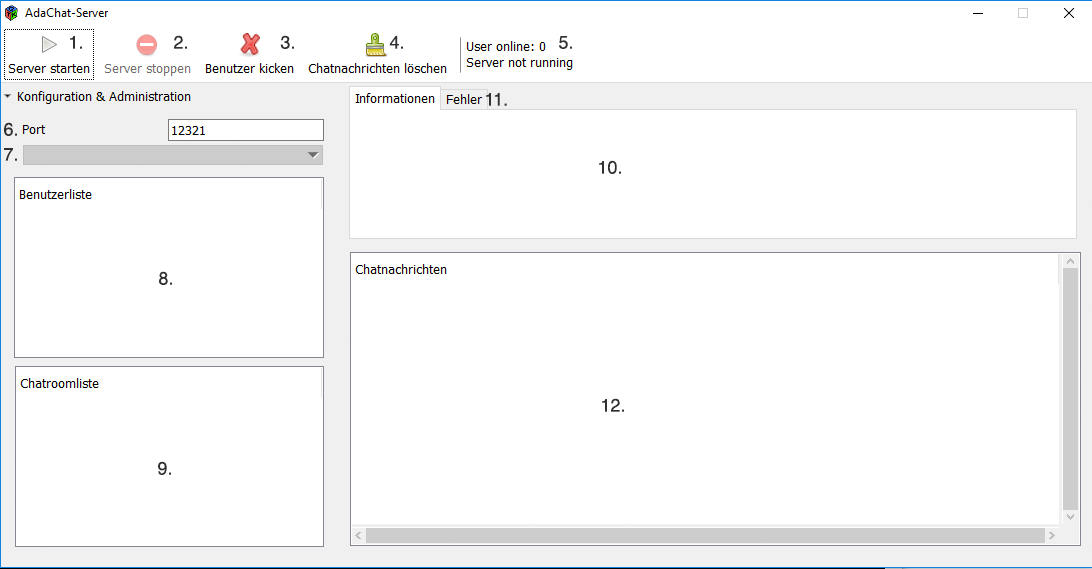
\includegraphics[width=1.0\linewidth]{img/Server_GUI.png}}
\end{minipage}
\vspace{0.5em}

\begin{enumerate}
	\item Mit diesem Button lässt sich der Server starten. Diese Schaltfläche ist nur aktiviert, wenn der Server nicht läuft.
	\item Mit diesem Button lässt sich der Server stoppen. Diese Schaltfläche ist nur aktiviert, wenn der Server läuft.
	\item Mit dieser Schaltfläche ist es möglich einen Benutzer aus dem Chat zu entfernen("kicken"). Der User, der entfernt werden soll, wird aus dem Drop-down-Menü unter \textit{7.} ausgewählt.
	\item Mit der Schaltfläche ist es möglich das Fenster mit den Chatnachrichten zu leeren.
	\item Hier wird der aktuelle Status des Servers angezeigt und die Anzahl der verbundenen Benutzer.
	\item In diesem Textfeld lässt sich der Port einstellen. Diese Einstellung lässt sich nicht zur Laufzeit verändern, sondern nur vor dem Start des Servers.
	\item In diesem Drop-down-Menü befinden sich alle Nutzer, die aktuell online sind. Wenn hier ein Benutzer ausgewählt wird, kann er über Schaltfläche \textit{3.} entfernt werden.
	\item Hier befindet sich die Benutzerliste. Dort erhalten Sie folgende Informationen über einen Benutzer:
		\begin{itemize}
			\item Benutzernamen
			\item IP-Adresse
			\item Seine Kontakte
			\item Die Chaträume, in denen er sich befindet
		\end{itemize}
	
	\item Hier finden Sie die Chaträume und die Benutzer, die sich in dem jeweiligen Raum befinden.
	\item In dem Feld unter dem Reiter \textit{Informationen} befinden sich Nachrichten des Servers über Ereignisse und Zustandsänderungen.
	\item In dem Feld unter dem Reiter \textit{Fehler} finden sich Fehlermeldungen des Servers.
	\item In diesem Feld befinden sich die Nachrichten der Benutzer in den einzelnen Chaträumen.
\end{enumerate}
\newpage
\subsection{Client}
Nach dem Server soll nun die Benutzeroberfläche der Clientanwendung beschrieben werden. Der Client besteht aus drei verschiedenen Oberflächen: Eine Loginoberfläche, ein Chatfenster und eine Übersichtsdarstellung.
\subsubsection{Loginoberfläche}
Die Loginoberfläche dient dazu einen vorhanden Benutzer beim Server anzumelden oder, falls der Benutzer noch nicht vorhanden ist, diesen zu registrieren.

\vspace{1em}
\begin{minipage}{\linewidth}
	\centering
	\frame{\includegraphics[width=0.5\linewidth]{img/Client_Login.png}}	
\end{minipage}
\vspace{0.5em}

\begin{enumerate}
	\item In diesem Feld wird die IP-Adresse des Rechners angegeben, auf dem der Server läuft.
	\item Hier wird der Port angegeben, auf dem der Server lauscht. Der Standardport ist 20000. 
	\item Hier wird der Benutzername eingegeben.
	\item In dieses Feld wird das Passwort eingegeben
	\item Mit einem Druck auf "Login" wird der Benutzer, falls die Benutzerdaten korrekt sind, beim Sever angemeldet.
	\item Mit einem Druck auf "Register" wird ein Benutzer mit den eingegebenen Benutzerdaten beim Server registriert.
\end{enumerate}
\subsubsection{Chatoberfläche}
Die Chatoberfläche ist das Fenster, in dem Chatnachrichten zwischen den Benutzern ausgetauscht werden.

\vspace{1em}
\begin{minipage}{\linewidth}
	\centering
	\frame{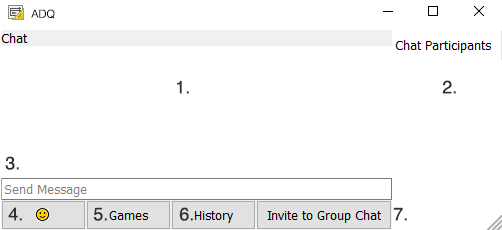
\includegraphics[width=0.8\linewidth]{img/client_chat.png}}	
\end{minipage}
\vspace{0.5em}

\begin{enumerate}
	\item In diesem Textfeld befindet sich eine Übersicht der bisher ausgetauschten Chatnachrichten.
	\item Hier befinden sich die Teilnehmer des Chats.
	\item In diesem Textfeld werden die Chatnachrichten eingegeben, die an die anderen Teilnehmer gesendet werden sollen.
	\item Über diesen Button lassen sich Smileys einfügen.
	\item Über diese Schaltfläche lassen sich Spiele mit den anderen Chatteilnehmern starten.
	\item Hierüber kann man sich vergangene Konversationen ansehen.
	\item Über diesen Button ist es möglich einen weiteren Teilnehmer zum Chat hinzuzufügen.
\end{enumerate}

\newpage
\section{GtkAda}
GtkAda ist eine Portierung des beliebten GTK+ Frameworks für die Sprache Ada. Es ist neben Qt eines der beliebtesten Frameworks zur Gestaltung von grafischen Oberflächen.  GTK+ wurde in C geschrieben und erschien 1998 das erste Mal. GtkAda implementiert alle Funktionen von GTK+ 3 und unterstützt ebenso die Entwicklung mit Glade, einem WYSIWYG für Oberflächen mit GTK. Diese lassen sich als XML exportieren und anschließend später mit GtkAda laden.

\newpage
\section{Hindernisse}
Im Folgenden sind die Problemstellungen aufgeführt, die in den Augen des Projektteams gravierend waren und die Entwicklung merkbar gehemmt haben.

\subsection{Dokumentation der Sprache Ada}
Das schwerwiegenste Problem, dass das Team über das ganze Projekt begleitet hat, war die unzureichende bis nicht vorhandene Dokumentation der Sprache Ada bzw. ihrer API.

Das Verhalten von bspw. Unterprogrammroutinen musste sich häufig allein durch die Bezeichnung und den Paramtern oder aus dem Kontext eines Programmierbeispiels von einem beliebigen Blog hergeleitet werden. Durch darauf folgendes mühsames und zeitintensives experimentieren konnte die fehlende Dokumentation dann meist kompensiert werden.

Es gibt zwar das Ada Reference Manual, welches sich jedoch meist nicht als sonderlich hilfreich erwies.

Jedoch muss man erwähnen, dass die Code-Qualität trotz alledem  unmittelbar darunter gelitten hat. Denn dadurch dass die Bibliotheksroutinen nicht ausreichend dokumentiert sind, kann unser Programm nur beschränkt auf z.B. Fehlersituationen oder anderweitiges situationsbedingtes Verhalten reagieren.

Abgesehen davon wird aus diesem Grund eine Beschäftigung mit der Spache über den Kurs hinaus kaum Anhang finden.

\subsection{Zirkuläre Abhängigkeiten}
Beim Aufbau von Datenstrukturen, wo die einen Bestandteil der anderen sind, traten des Öfteren zirkuläre Abhängigkeitsprobleme auf. Es wurden zwei Methoden verwendet, um diese Probleme zu beseitigen. Zum einen ist es möglich, alle Datentypen in einer gemeinsamen Spezifikationsdatei (.ads) zu definieren. Somit ist es nicht notwendig, andere Spezifikationen einzubinden, es existieren keine Abhängigkeiten nach außen. Da dies allerdings zu einer sehr unübersichtlichen Projektstruktur führt, wurde wenn möglich die umgekehrte Methodik verwendet und unabhängige Datenstrukturen jeweils in ihrem eigenen File beschrieben, welches dann von den zwei nutzenden Strukturen referenziert wird.

Ada 2005 bietet zur Beseitigung von zirkulären Abhängigkeiten die \glqq{}limited with\grqq{}-Klausel an. Da dies aber nur eine unvollständige Sicht auf das somit eingebundene Paket oder den somit eingebundenen Typen liefert, konnte dies nicht immer verwendet werden (siehe \url{http://www.adaic.org/resources/add_content/standards/05rat/html/Rat-1-3-3.html}).

%link gescheit einbinden

Rekursive Datenstrukturen - zum Beispiel ein Benutzer, der seine Kontakte in einer Liste aus Benutzern speichert - können in Ada nur definiert werden, in dem der Datentyp zuvor als unvollständiger Typ deklariert wurde. Dieses Prinzip ist zwar aus anderen Programmiersprachen wie C bekannt, zerstückelt den Quellcode aber dennoch und ist somit ein weiterer Nachteil dieser Sprache.

%Da in Ada ein Bezeichner vor dessen Verwendung deklariert werden muss, war es nicht einfach %Protected Types, Types, Pointer Types, Interfaces frei miteinander zu kombinieren. 
%was ist hier gemeint?

Außerdem war verwunderlich, dass das Einbinden von Spezifikationsdateien in eine Bodydatei (.adb) ein anderes Folgeverhalten bezüglich der zirkulären Abhängigkeiten aufweisen kann, als wenn diese in die dem Body zugehörige Spezifikationsdatei eingebunden werden. Manche zirkuläre Abhängigkeit konnte nur so aufgelöst werden.

\subsection{Arbeiten mit GtkAda}
 Während der Arbeit mit GtkAda  traten einige Dinge besonders negativ in den Vordergrund, die wir nun erläutern möchten.

\begin{enumerate}
	\item \textbf{Dokumentation}	\hfill \\
	Wie auch schon Ada im Allgemeinen ist die Dokumentations- und Informationslage zu GtkAda dürftig. Es gibt keine offizielle Dokumentation und wenige Beispiele, die leider auch meistens nur einen kleinen Umfang haben und nur einzelne Komponenten abdecken, nicht jedoch mehrere Komponenten im Zusammenspiel. Falls man nach Lösungen zu bestimmten Fragestellungen sucht, findet man meistens keine GtkAda spezifische Antwort, sondern muss oftmals Lösungen aus anderen Programmiersprachen (Python oder C) auf Ada übertragen. Dies lässt sich jedoch oftmals nicht ohne Weiteres umsetzen, da GtkAda manche Dinge anders handhabt bzw. benennt (beispielsweise bei der Nutzung von \textit{Gtk\textunderscore Tree\textunderscore Model} und \textit{Gtk\textunderscore Tree\textunderscore Store}).
	
	\item \textbf{Glade} \hfill \\
	Glade ist ein Tool, um sich grafische Oberflächen schnell zu erstellen und diese in eine \textit{.glade} Datei zu exportieren. Dabei handelt es sich um eine XML-strukturierte Datei, die die Oberfläche und Voreinstellungen enthält. Das Problem an Glade ist leider, das es nicht stabil läuft und die Portierungen für Windows und Mac OS X zu Darstellungsfehlern und Performanceeinbrüchen neigen.
	
	\item \textbf{GtkAda \& Tasks }\hfill \\	
	Ebenfalls erlaubt es GtkAda nicht, aus einem Task, welcher nicht der GTK-Main-Task ist, dynamisch neue Fenster zu generieren ohne abzustürzen. Dem Öffnen eines neuen Chatfensters, beispielsweise nachdem eine Chat-Nachricht eingegangen ist, muss daher eine Benutzerinteraktion mit der grafischen Oberfläche vorausgehen. Diese Interaktion wird vom GTK-Main-Task verarbeitet, und führt dadurch nicht zum Absturz des Programms.
	
	Durch diese Unpraktikabilität des Frameworks muss der Benutzer durch das unkritische Transformieren eines bestehenden GUI-Elements (in diesem Fall das Fettdrucken des Namens des schreibenden Kontakts) darauf aufmerksam gemacht werden, dass eine Oberflächeninteraktion gefordert ist.
	
	Allgemein gilt die GTK-Implementierung für Ada unter Windows als nicht task-sicher, für andere Betriebssysteme existieren mehr oder minder aufwändige Workarounds, um das simultane Zugreifen auf diverse Gdk-Routinen zu erlauben (siehe \url{http://docs.adacore.com/gtkada-docs/gtkada_ug/_build/html/tasking.html}).
	
	\end{enumerate}


\pagebreak



% ----------------------------------------------------------------------------------------------------------
% Literatur
% ----------------------------------------------------------------------------------------------------------
\renewcommand\refname{Quellenverzeichnis}

%\bibliographystyle{alphadin}
%\nocite{*}
%\bibliography{bib/lit.bib}


\end{document}
